\documentclass[aspectratio=169,10pt]{beamer}
\usetheme{metropolis}
\usepackage{listings,xcolor,booktabs,amsmath,amssymb,mathtools,stmaryrd}
\usepackage{tikz,tikz-cd}
\providecommand{\llbracket}{\lBrack}
\providecommand{\rrbracket}{\rBrack}
\usetikzlibrary{arrows.meta,positioning,calc,decorations.pathmorphing,shapes}

\definecolor{codebg}{HTML}{F5F5F5}
\definecolor{good}{HTML}{2E7D32}
\definecolor{meh}{HTML}{E65100}
\definecolor{honest}{HTML}{1565C0}
\definecolor{mathblue}{HTML}{1A237E}
\definecolor{defgreen}{HTML}{1B5E20}
\definecolor{exred}{HTML}{B71C1C}

\lstset{
  basicstyle=\ttfamily\tiny,
  backgroundcolor=\color{codebg},
  frame=single, framerule=0.3pt,
  columns=fullflexible, keepspaces=true, language=Python,
  keywordstyle=\color{blue!70!black},
  commentstyle=\color{gray},
  stringstyle=\color{red!60!black},
  breaklines=true,
  aboveskip=0.4em,belowskip=0.2em,
}

\setbeamertemplate{frametitle}{\vspace{-0.2em}\insertframetitle\vspace{-0.3em}}
\setbeamersize{text margin left=7mm, text margin right=7mm}

\newcommand{\yes}{\textcolor{good}{\checkmark}}
\newcommand{\no}{\textcolor{meh}{$\times$}}
\newcommand{\Fscr}{\mathcal{F}}
\newcommand{\Gscr}{\mathcal{G}}
\newcommand{\Oscr}{\mathcal{O}}
\newcommand{\Uscr}{\mathcal{U}}
\newcommand{\Iso}{\mathrm{Iso}}
\newcommand{\Sem}{\mathrm{Sem}}
\newcommand{\op}{\mathrm{op}}
\newcommand{\Hom}{\mathrm{Hom}}
\newcommand{\im}{\operatorname{im}}
\newcommand{\rk}{\operatorname{rk}}
\newcommand{\id}{\mathrm{id}}
\newcommand{\Ob}{\mathrm{Ob}}
\newcommand{\Poset}{\mathbf{Poset}}
\newcommand{\Set}{\mathbf{Set}}
\newcommand{\Ab}{\mathbf{Ab}}
\newcommand{\Cat}{\mathbf{Cat}}
\newcommand{\Open}{\mathrm{Open}}

\title{Background for ``What Sheaf Theory Actually Gets You''}
\subtitle{200 slides on PL, Sheaf Theory, and Cohomology}
\author{}
\date{}

\begin{document}

% ╔═══════════════════════════════════════════════════════════════════════════╗
% ║  PART I: PROGRAMMING LANGUAGE FOUNDATIONS (Slides 1-60)                  ║
% ╚═══════════════════════════════════════════════════════════════════════════╝

% ── SLIDE 1 ──────────────────────────────────────────────────
\begin{frame}[plain]
\vspace{1.5cm}
\begin{center}
{\Large\textbf{Background for\\``What Sheaf Theory Actually Gets You''}}\\[0.5em]
{\normalsize PL Foundations $\bullet$ Sheaf Theory $\bullet$ Cohomology}\\[1em]
{\small\textit{Everything you need to present the deppy\_honest\_comparison\\
confidently, starting from first principles.}}
\end{center}
\end{frame}

% ── SLIDE 2 ──────────────────────────────────────────────────
\begin{frame}{Roadmap}
\begin{enumerate}
  \item \textbf{Part I} (Slides 1--60): PL foundations---types, abstract interpretation, refinement types, dependent types, verification conditions
  \item \textbf{Part II} (Slides 61--120): Sheaf theory---categories, presheaves, sheaves, Grothendieck topologies, sites, descent
  \item \textbf{Part III} (Slides 121--170): Cohomology---cochain complexes, \v{C}ech cohomology, $H^0$/$H^1$, Mayer-Vietoris, obstructions
  \item \textbf{Part IV} (Slides 171--200): Connecting it all---how deppy uses sheaves for bug-finding, equivalence, and spec-checking
\end{enumerate}

\vspace{0.5em}
\textcolor{honest}{\textbf{Goal:}} After these slides, every symbol and claim in the 10-slide presentation should feel natural.
\end{frame}

% ══════════════════════════════════════════════════════════════
% SECTION: What is a Type System?
% ══════════════════════════════════════════════════════════════

\begin{frame}[plain]
\begin{center}
\vspace{2cm}
{\Huge\textbf{Part I}}\\[0.3em]
{\Large Programming Language Foundations}\\[1em]
{\normalsize Types $\to$ Abstract Interpretation $\to$ Refinement Types $\to$\\
 Dependent Types $\to$ Verification Conditions}
\end{center}
\end{frame}

% ── SLIDE 4 ──────────────────────────────────────────────────
\begin{frame}{What Is a Type?}
\textbf{Informal:} A type classifies values by the operations they support.

\vspace{0.5em}
\textbf{Formal (set-theoretic):} A type $\tau$ denotes a set $\llbracket \tau \rrbracket$ of values.
\begin{itemize}
  \item $\llbracket \texttt{int} \rrbracket = \mathbb{Z}$
  \item $\llbracket \texttt{bool} \rrbracket = \{\texttt{True}, \texttt{False}\}$
  \item $\llbracket \texttt{int} \to \texttt{int} \rrbracket = \mathbb{Z} \to \mathbb{Z}$
\end{itemize}

\vspace{0.5em}
\textbf{Why types?}
\begin{enumerate}
  \item \emph{Safety}: prevent nonsensical operations ($\texttt{"hello"} + 3$)
  \item \emph{Abstraction}: hide implementation details
  \item \emph{Documentation}: machine-checked contracts
\end{enumerate}
\end{frame}

% ── SLIDE 5 ──────────────────────────────────────────────────
\begin{frame}{Type Judgments}
A \textbf{typing judgment} has the form:
\[
\Gamma \vdash e : \tau
\]
Read: ``In context $\Gamma$, expression $e$ has type $\tau$.''

\vspace{0.3em}
\textbf{Context} $\Gamma$ is a list of variable-type bindings: $x_1:\tau_1, \ldots, x_n:\tau_n$.

\vspace{0.3em}
\textbf{Example rules:}
\[
\frac{\Gamma \vdash e_1 : \texttt{int} \quad \Gamma \vdash e_2 : \texttt{int}}
     {\Gamma \vdash e_1 + e_2 : \texttt{int}} \;\text{(T-Add)}
\qquad
\frac{\Gamma, x:\tau_1 \vdash e : \tau_2}
     {\Gamma \vdash \lambda x.\, e : \tau_1 \to \tau_2} \;\text{(T-Abs)}
\]
\end{frame}

% ── SLIDE 6 ──────────────────────────────────────────────────
\begin{frame}{Type Soundness}
\textbf{The fundamental theorem of type systems:}

\begin{block}{Type Soundness (Milner, 1978; Wright \& Felleisen, 1994)}
Well-typed programs do not go wrong.\\[0.3em]
Formally: \emph{Progress} + \emph{Preservation}.
\end{block}

\vspace{0.3em}
\begin{description}
  \item[Progress] If $\vdash e : \tau$, then either $e$ is a value or $e \to e'$.
  \item[Preservation] If $\vdash e : \tau$ and $e \to e'$, then $\vdash e' : \tau$.
\end{description}

\vspace{0.3em}
\textbf{Why this matters for deppy:} The sheaf gluing condition is a \emph{generalized} soundness check---local type assignments ``glue'' iff the program is well-typed.
\end{frame}

% ── SLIDE 7 ──────────────────────────────────────────────────
\begin{frame}{The Curry-Howard Correspondence}
\begin{center}
\renewcommand{\arraystretch}{1.4}
\begin{tabular}{@{}ll@{}}
\toprule
\textbf{Logic} & \textbf{Type Theory} \\
\midrule
Proposition $P$ & Type $\tau$ \\
Proof of $P$ & Term $e : \tau$ \\
$P \Rightarrow Q$ & Function type $\tau_1 \to \tau_2$ \\
$P \wedge Q$ & Product type $\tau_1 \times \tau_2$ \\
$P \vee Q$ & Sum type $\tau_1 + \tau_2$ \\
$\forall x.\, P(x)$ & Dependent product $\Pi_{x:\tau_1} \tau_2(x)$ \\
$\exists x.\, P(x)$ & Dependent sum $\Sigma_{x:\tau_1} \tau_2(x)$ \\
\bottomrule
\end{tabular}
\end{center}

\vspace{0.3em}
\textbf{Key insight:} Type checking = proof checking. Deppy's ``verification conditions'' are propositions; solving them is proving them.
\end{frame}

% ── SLIDE 8 ──────────────────────────────────────────────────
\begin{frame}{Simple Types vs.\ Rich Types}
\textbf{Simple types} (Java, Go, C):
\begin{itemize}
  \item $\texttt{int}$, $\texttt{String}$, $\texttt{List<T>}$
  \item Can catch: wrong argument count, type mismatches
  \item Cannot catch: division by zero, array out of bounds, null dereference
\end{itemize}

\vspace{0.5em}
\textbf{Richer type systems} add expressive power:
\begin{enumerate}
  \item \textbf{Generics/Parametric polymorphism}: $\forall \alpha.\, \alpha \to \alpha$
  \item \textbf{Refinement types}: $\{x : \texttt{int} \mid x > 0\}$
  \item \textbf{Dependent types}: $\texttt{Vec}(n) \to \texttt{Vec}(n)$
  \item \textbf{Linear types}: use each value exactly once
\end{enumerate}

\vspace{0.3em}
Deppy operates at levels 2--3: refinement + dependent types for Python.
\end{frame}

% ── SLIDE 9 ──────────────────────────────────────────────────
\begin{frame}{What Is Abstract Interpretation?}
\begin{block}{Definition (Cousot \& Cousot, 1977)}
Abstract interpretation computes an \emph{over-approximation} of all possible runtime states by executing the program on an \emph{abstract domain} instead of concrete values.
\end{block}

\vspace{0.3em}
\textbf{Concrete domain:} $(\mathcal{P}(\mathbb{Z}), \subseteq)$ --- sets of integers.\\
\textbf{Abstract domain:} e.g., intervals $[a, b]$, signs $\{-, 0, +\}$, octagons.

\vspace{0.5em}
\textbf{Galois connection:}
\[
\alpha : \mathcal{P}(\mathbb{Z}) \rightleftharpoons \widehat{D} : \gamma
\qquad
\alpha(S) = \text{best abstraction of } S
\qquad
\gamma(\hat{d}) = \text{concrete values represented by } \hat{d}
\]
\end{frame}

% ── SLIDE 10 ─────────────────────────────────────────────────
\begin{frame}[fragile]{Abstract Interpretation: Interval Example}
\begin{lstlisting}
def f(x: int, y: int):
    z = x + y       # z in [x+y, x+y]
    if z > 0:
        w = 100 / z  # safe: z > 0
    else:
        w = z - 1    # z <= 0, so w <= -1
    return w
\end{lstlisting}

\textbf{Interval analysis:}
\begin{itemize}
  \item After branch $z > 0$: $z \in [1, +\infty)$ --- division safe
  \item After branch $z \leq 0$: $z \in (-\infty, 0]$ --- no division
\end{itemize}

\vspace{0.3em}
\textbf{The good:} Fully automatic, sound, scales to large programs.\\
\textbf{The bad:} Imprecise (joins lose information), requires widening for loops.
\end{frame}

% ── SLIDE 11 ─────────────────────────────────────────────────
\begin{frame}{Fixpoints and Widening}
\textbf{Loops} require computing a fixpoint of the abstract transfer function:
\[
\hat{d}^{(n+1)} = f^\sharp(\hat{d}^{(n)}) \sqcup \hat{d}^{(n)}
\]

\textbf{Problem:} Ascending chains may not stabilize (e.g., $[0,1], [0,2], [0,3], \ldots$).

\vspace{0.3em}
\textbf{Widening} $\nabla$ forces convergence by jumping ahead:
\[
\hat{d}^{(n+1)} = \hat{d}^{(n)} \;\nabla\; f^\sharp(\hat{d}^{(n)})
\]

\textbf{Cost:} Widening loses precision \emph{non-monotonically}---you might overshoot and never recover.

\vspace{0.5em}
\textcolor{honest}{\textbf{This is exactly what the sheaf approach avoids:}} checking \emph{agreement} on overlaps doesn't require computing a global fixpoint.
\end{frame}

% ── SLIDE 12 ─────────────────────────────────────────────────
\begin{frame}{The Global Fixpoint Problem}
\textbf{Standard abstract interpretation} computes a \emph{single global abstract state}:

\begin{center}
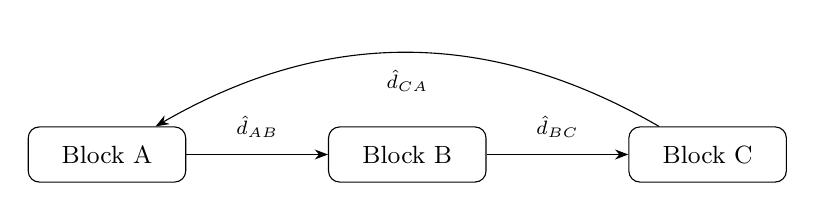
\begin{tikzpicture}[node distance=1.8cm, >=Stealth, every node/.style={draw, rounded corners, minimum width=2cm, minimum height=0.7cm, font=\small}]
  \node (a) {Block A};
  \node (b) [right=of a] {Block B};
  \node (c) [right=of b] {Block C};
  \draw[->] (a) -- node[above, draw=none, font=\scriptsize] {$\hat{d}_{AB}$} (b);
  \draw[->] (b) -- node[above, draw=none, font=\scriptsize] {$\hat{d}_{BC}$} (c);
  \draw[->, bend right=30] (c) to node[below, draw=none, font=\scriptsize] {$\hat{d}_{CA}$} (a);
\end{tikzpicture}
\end{center}

With $|D|$ = domain size and $k$ = program variables:
\[
\text{Cost} = \mathcal{O}(|D|^k) \quad\text{per fixpoint iteration}
\]

\textbf{Pain points:}
\begin{itemize}
  \item Cost is \emph{exponential} in number of tracked variables
  \item Widening loses precision globally
  \item A single imprecise join poisons the entire analysis
\end{itemize}
\end{frame}

% ── SLIDE 13 ─────────────────────────────────────────────────
\begin{frame}{Refinement Types: The Idea}
\textbf{Refinement types} attach logical predicates to base types:
\[
\{x : \tau \mid \varphi(x)\}
\]

\textbf{Examples:}
\begin{itemize}
  \item $\{x : \texttt{int} \mid x > 0\}$ --- positive integers
  \item $\{x : \texttt{int} \mid x \neq 0\}$ --- nonzero integers (safe divisors)
  \item $\{a : \texttt{List}[\texttt{int}] \mid \texttt{len}(a) = n\}$ --- length-indexed lists
\end{itemize}

\vspace{0.3em}
\textbf{Subtyping rule:}
\[
\frac{\forall x.\; \varphi_1(x) \Rightarrow \varphi_2(x)}
     {\{x:\tau \mid \varphi_1\} <: \{x:\tau \mid \varphi_2\}}
\]

Checking subtyping = checking logical implication = \textbf{SMT query}.
\end{frame}

% ── SLIDE 14 ─────────────────────────────────────────────────
\begin{frame}[fragile]{Refinement Types: Liquid Haskell Example}
\begin{lstlisting}[language=Haskell]
{-@ divide :: Int -> {v:Int | v /= 0} -> Int @-}
divide :: Int -> Int -> Int
divide x y = x `div` y

{-@ average :: {v:[Int] | len v > 0} -> Int @-}
average :: [Int] -> Int
average xs = divide (sum xs) (length xs)
\end{lstlisting}

\vspace{0.3em}
Liquid Haskell generates a \textbf{verification condition} (VC):
\[
\texttt{len}(xs) > 0 \;\Rightarrow\; \texttt{length}(xs) \neq 0
\]
and sends it to Z3. If SAT (valid): the program is safe.

\vspace{0.5em}
\textbf{Limitation:} One monolithic VC per function. Deppy's sheaf approach factors this into per-site VCs.
\end{frame}

% ── SLIDE 15 ─────────────────────────────────────────────────
\begin{frame}{Dependent Types: The Full Power}
\textbf{Dependent types} allow types to depend on \emph{values}:
\[
\Pi_{n:\mathbb{N}}.\; \texttt{Vec}(n) \to \texttt{Vec}(n)
\]
``For all $n$, takes a vector of length $n$, returns a vector of length $n$.''

\vspace{0.3em}
\textbf{Key constructs:}
\begin{description}
  \item[$\Pi$-type] (dependent function): $\Pi_{x:A} B(x)$ --- generalization of $A \to B$
  \item[$\Sigma$-type] (dependent pair): $\Sigma_{x:A} B(x)$ --- generalization of $A \times B$
  \item[Id-type] (identity/equality): $\mathrm{Id}_A(x, y)$ --- proof that $x = y$ in $A$
\end{description}

\vspace{0.3em}
Refinement types are a \emph{restricted} form: $\{x : \tau \mid \varphi\} \cong \Sigma_{x:\tau} \varphi(x)$ where $\varphi$ is decidable.
\end{frame}

% ── SLIDE 16 ─────────────────────────────────────────────────
\begin{frame}{Dependent Types in Practice}
\textbf{Full dependent types} (Coq, Agda, Lean, Idris):
\begin{itemize}
  \item Extremely expressive: can state any mathematical property
  \item Type checking is undecidable in general (requires user-provided proofs)
  \item Manual proof burden is significant
\end{itemize}

\vspace{0.5em}
\textbf{Deppy's sweet spot:} Dependent types for Python, but with \emph{automated} proof via SMT.
\begin{itemize}
  \item User writes: \texttt{@deppy.requires(lambda x: x > 0)}
  \item Deppy infers refinements, generates VCs, calls Z3
  \item No manual proofs needed for decidable fragments
\end{itemize}

\vspace{0.3em}
\textbf{Deppy's identity type} (\texttt{IdentityType}): used for equivalence proofs between implementations.
\end{frame}

% ── SLIDE 17 ─────────────────────────────────────────────────
\begin{frame}{Verification Conditions (VCs)}
A \textbf{verification condition} is a logical formula whose validity implies program correctness.

\vspace{0.3em}
\textbf{Standard pipeline:}
\[
\text{Source code} \;\xrightarrow{\text{VC gen}}\; \text{Logical formula}
\;\xrightarrow{\text{SMT solver}}\; \text{Valid/Invalid + counterexample}
\]

\vspace{0.3em}
\textbf{Example:} For function with precondition $P$ and postcondition $Q$:
\[
\text{VC} = \forall \vec{x}.\; P(\vec{x}) \;\Rightarrow\; \text{wp}(\text{body}, Q)(\vec{x})
\]
where $\text{wp}$ is the weakest precondition transformer.

\vspace{0.3em}
\textbf{Tools:} Dafny, F*, Liquid Haskell, Why3, Frama-C all generate VCs.
Deppy does too---but \emph{decomposes} them via the sheaf cover.
\end{frame}

% ── SLIDE 18 ─────────────────────────────────────────────────
\begin{frame}{SMT Solvers: The Decision Engine}
\textbf{Satisfiability Modulo Theories} (SMT) solvers decide:
\[
\exists \vec{x}.\; \varphi(\vec{x}) \quad\text{over theories } T_1, \ldots, T_k
\]

\textbf{Common theories:}
\begin{description}
  \item[QF\_LIA] Quantifier-free linear integer arithmetic (decidable, in NP)
  \item[QF\_LRA] Quantifier-free linear real arithmetic (decidable, in P)
  \item[QF\_NIA] Quantifier-free nonlinear integer arithmetic (undecidable!)
  \item[QF\_BV] Bit-vectors (decidable, NP-complete)
  \item[QF\_UF] Uninterpreted functions with equality (decidable)
\end{description}

\vspace{0.3em}
\textbf{Key for deppy:} Each local VC is typically in QF\_LIA or QF\_UF --- cheap to solve. The \emph{locality} of sheaf queries keeps us in decidable fragments.
\end{frame}

% ── SLIDE 19 ─────────────────────────────────────────────────
\begin{frame}{Nelson-Oppen Theory Combination}
\textbf{Problem:} Real VCs mix theories (arithmetic + arrays + functions).

\vspace{0.3em}
\textbf{Nelson-Oppen (1979):} Combine decision procedures for disjoint-signature theories.

\textbf{Requirements:}
\begin{enumerate}
  \item Theories share only equality
  \item Each theory is \emph{stably infinite} (infinite models exist)
  \item Each theory is decidable individually
\end{enumerate}

\textbf{Algorithm:} Propagate equalities between shared variables until fixpoint.

\vspace{0.5em}
\textbf{Deppy uses this:} The \texttt{theory\_interface.py} module enforces signature disjointness for theory combination in the solver backend. Tinelli-Zarba (2005) extends Nelson-Oppen to non-stably-infinite theories.
\end{frame}

% ── SLIDE 20 ─────────────────────────────────────────────────
\begin{frame}{CEGAR: Counterexample-Guided Abstraction Refinement}
\textbf{CEGAR} (Clarke et al., 2000) iteratively refines an abstraction:

\begin{center}
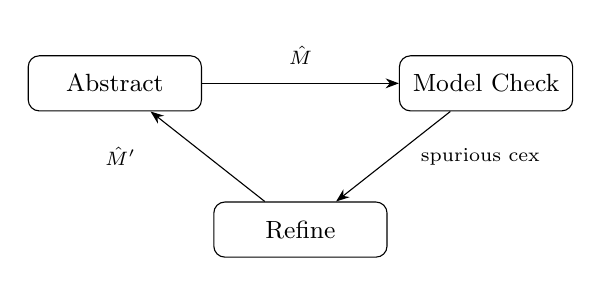
\begin{tikzpicture}[node distance=2.5cm, >=Stealth, every node/.style={draw, rounded corners, minimum width=2.2cm, minimum height=0.7cm, font=\small}]
  \node (abs) {Abstract};
  \node (check) [right=of abs] {Model Check};
  \node (ref) [below=1.5cm of $(abs)!0.5!(check)$] {Refine};
  \draw[->] (abs) -- node[above, draw=none, font=\scriptsize] {$\hat{M}$} (check);
  \draw[->] (check) -- node[right, draw=none, font=\scriptsize] {spurious cex} (ref);
  \draw[->] (ref) -- node[left, draw=none, font=\scriptsize] {$\hat{M}'$} (abs);
\end{tikzpicture}
\end{center}

\vspace{0.3em}
\begin{enumerate}
  \item Start with coarse abstraction
  \item Check property --- if holds, done
  \item If counterexample is spurious, refine abstraction
  \item Repeat
\end{enumerate}

\textbf{Deppy's CEGAR loop:} uses unsat cores from Z3 to identify which predicates to add per iteration.
\end{frame}

% ── SLIDE 21 ─────────────────────────────────────────────────
\begin{frame}{Control Flow Graphs and Basic Blocks}
\textbf{Control Flow Graph (CFG):} Nodes = basic blocks, edges = control flow.

A \textbf{basic block} is a maximal sequence of instructions with:
\begin{itemize}
  \item One entry point (first instruction)
  \item One exit point (last instruction)
  \item No branches in the middle
\end{itemize}

\vspace{0.3em}
\textbf{Why CFGs matter for deppy:}
\begin{itemize}
  \item Each basic block (or branch arm) becomes an \emph{observation site}
  \item Edges between blocks become \emph{overlaps} in the cover
  \item The CFG structure \emph{is} the topological space on which the sheaf lives
\end{itemize}
\end{frame}

% ── SLIDE 22 ─────────────────────────────────────────────────
\begin{frame}{SSA Form and Value Lineage}
\textbf{Static Single Assignment (SSA):} Every variable is assigned exactly once.

\begin{center}
\begin{tabular}{@{}l@{\qquad$\to$\qquad}l@{}}
\texttt{x = 1; x = x + 1} & \texttt{x\_1 = 1; x\_2 = x\_1 + 1}
\end{tabular}
\end{center}

At join points, use $\phi$-functions: $\texttt{x\_3} = \phi(\texttt{x\_1}, \texttt{x\_2})$.

\vspace{0.3em}
\textbf{SSA in deppy:}
\begin{itemize}
  \item Each SSA value is a potential \textbf{site} (kind: \texttt{SSA\_VALUE})
  \item $\phi$-nodes are natural \textbf{overlap} points between branches
  \item The \texttt{value\_lineage.py} module tracks which sites share which SSA values
  \item The \texttt{phi\_merge.py} module handles merging sections at join points
\end{itemize}
\end{frame}

% ── SLIDE 23 ─────────────────────────────────────────────────
\begin{frame}{Dataflow Analysis}
\textbf{Dataflow analysis} computes facts that hold at each program point.

\textbf{Framework:} $(L, \sqsubseteq, \sqcup, \sqcap, \bot, \top)$ --- a lattice of dataflow facts.

\vspace{0.3em}
\textbf{Transfer function:} $f_B : L \to L$ for each basic block $B$.
\textbf{Join:} $\text{in}(B) = \bigsqcup_{P \in \text{pred}(B)} \text{out}(P)$.

\vspace{0.5em}
\textbf{Classic analyses:}
\begin{itemize}
  \item Reaching definitions (which assignments reach which uses)
  \item Live variables (which variables are read before next write)
  \item Available expressions (which expressions are already computed)
\end{itemize}

\vspace{0.3em}
\textbf{Connection to deppy:} Dataflow = ``pushing information forward/backward.'' Deppy replaces the global fixpoint with \emph{local section inference + gluing check}.
\end{frame}

% ── SLIDE 24 ─────────────────────────────────────────────────
\begin{frame}{Interprocedural Analysis}
\textbf{Problem:} Function calls cross procedure boundaries.

\textbf{Approaches:}
\begin{enumerate}
  \item \textbf{Inlining}: Expand callees. Exponential blowup.
  \item \textbf{Summaries}: Compute $f : \text{input type} \to \text{output type}$ once, reuse.
  \item \textbf{Context sensitivity}: Distinguish call sites ($k$-CFA, object sensitivity).
\end{enumerate}

\vspace{0.5em}
\textbf{Deppy's approach:}
\begin{itemize}
  \item \texttt{summary\_propagation.py}: Computes function summaries as sections
  \item \texttt{section\_transport.py}: Transports sections across call boundaries
  \item \texttt{context\_sensitivity.py}: Distinguishes calling contexts
  \item Result: interprocedural analysis as \textbf{section transport on the presheaf}
\end{itemize}
\end{frame}

% ── SLIDE 25 ─────────────────────────────────────────────────
\begin{frame}{What Is Modular Verification?}
\textbf{Modular verification} checks each module independently, then composes results.

\vspace{0.3em}
\textbf{The compositionality problem:}
\begin{itemize}
  \item Module $A$ passes its own spec
  \item Module $B$ passes its own spec
  \item Does $A \circ B$ pass the combined spec?
\end{itemize}

\vspace{0.3em}
\textbf{Standard answer:} If interfaces match --- yes (\emph{sound but incomplete}).

\textbf{Sheaf answer:} If $H^1 = 0$ --- yes (\emph{sound \textbf{and} complete} for the cover).

\vspace{0.5em}
\textcolor{honest}{\textbf{This is the key upgrade:}} Standard modular checking can reject \emph{equivalent} programs with non-matching interfaces. The sheaf approach doesn't.
\end{frame}

% ── SLIDE 26 ─────────────────────────────────────────────────
\begin{frame}{Program Equivalence}
\textbf{Question:} Do two programs $f$ and $g$ compute the same function?

\vspace{0.3em}
\textbf{Why hard:}
\begin{itemize}
  \item Undecidable in general (Rice's theorem)
  \item Even for terminating programs: exponential state spaces
\end{itemize}

\textbf{Approaches:}
\begin{enumerate}
  \item \textbf{Bisimulation}: lockstep simulation (exponential)
  \item \textbf{Translation validation}: check compiler output matches source
  \item \textbf{Relational verification}: prove $\forall \vec{x}.\; f(\vec{x}) = g(\vec{x})$
\end{enumerate}

\vspace{0.3em}
\textbf{Deppy's approach:} Decompose the equivalence check into \emph{local} checks on sites, then glue via \v{C}ech cohomology. Exponential $\to$ polynomial when variables partition.
\end{frame}

% ── SLIDE 27 ─────────────────────────────────────────────────
\begin{frame}{Bisimulation}
\textbf{Bisimulation} is the gold standard for behavioral equivalence.

\vspace{0.3em}
\textbf{Definition:} A relation $R \subseteq S_f \times S_g$ is a \emph{bisimulation} if for all $(s, t) \in R$:
\begin{enumerate}
  \item If $s \xrightarrow{a} s'$, then $\exists t'$ such that $t \xrightarrow{a} t'$ and $(s', t') \in R$.
  \item Symmetrically for transitions from $t$.
\end{enumerate}

\vspace{0.3em}
\textbf{Cost:} State space is $|S_f| \times |S_g|$.
With $k$ variables of domain size $d$: state space $= d^k \times d^k = d^{2k}$.

\vspace{0.3em}
\textbf{The deppy win:} Decompose into $m$ sites each touching $k/m$ variables.
Cost: $m \cdot d^{2k/m} \ll d^{2k}$ for $m > 1$.
\end{frame}

% ── SLIDE 28 ─────────────────────────────────────────────────
\begin{frame}{What Astree / Infer / Pyright Can Do}
\textbf{Industrial analyzers} deppy compares against:

\vspace{0.3em}
\renewcommand{\arraystretch}{1.3}
\begin{tabular}{@{}lp{8cm}@{}}
\toprule
\textbf{Tool} & \textbf{Approach} \\
\midrule
\textbf{Astr\'ee} & Abstract interpretation (intervals, octagons, polyhedra). Proves \emph{absence} of runtime errors. No user annotations. \\
\textbf{Infer} & Bi-abduction (separation logic). Memory safety, null pointer, data races. \\
\textbf{Pyright/Mypy} & Type inference for Python. Structural, no refinement predicates. \\
\textbf{Liquid Haskell} & Refinement types + SMT. Powerful but requires type annotations. \\
\bottomrule
\end{tabular}

\vspace{0.3em}
\textbf{What none of them provide:}
\begin{itemize}
  \item Compositional obstruction counting ($\rk H^1$)
  \item Behavioral equivalence with completeness guarantees
  \item Structured soundness certificates ($H^0 + H^1$)
\end{itemize}
\end{frame}

% ── SLIDE 29 ─────────────────────────────────────────────────
\begin{frame}{Deppy's Pipeline Overview}
\begin{center}
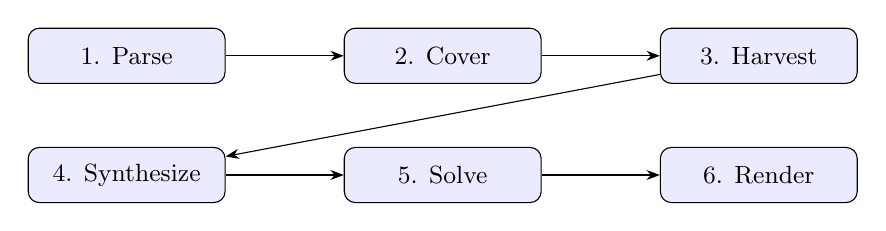
\begin{tikzpicture}[node distance=1.5cm, >=Stealth,
  stage/.style={draw, rounded corners, fill=blue!8, minimum width=2.5cm, minimum height=0.7cm, font=\small}]
  \node[stage] (parse) {1. Parse};
  \node[stage, right=of parse] (cover) {2. Cover};
  \node[stage, right=of cover] (harvest) {3. Harvest};
  \node[stage, below=0.8cm of parse] (synth) {4. Synthesize};
  \node[stage, right=of synth] (solve) {5. Solve};
  \node[stage, right=of solve] (render) {6. Render};
  \draw[->] (parse) -- (cover);
  \draw[->] (cover) -- (harvest);
  \draw[->] (harvest) -- (synth);
  \draw[->] (synth) -- (solve);
  \draw[->] (solve) -- (render);
\end{tikzpicture}
\end{center}

\begin{enumerate}\small
  \item \textbf{Parse}: Python AST $\to$ IR (core terms)
  \item \textbf{Cover}: Build observation sites + overlaps (the topological space)
  \item \textbf{Harvest}: Infer local sections at each site (the presheaf)
  \item \textbf{Synthesize}: Forward/backward section propagation (kernel)
  \item \textbf{Solve}: Check gluing condition, extract $H^1$ obstructions
  \item \textbf{Render}: Diagnostics, repair suggestions, SARIF export
\end{enumerate}
\end{frame}

% ── SLIDE 30 ─────────────────────────────────────────────────
\begin{frame}{Deppy's 14 Site Families}
\renewcommand{\arraystretch}{1.15}
\footnotesize
\begin{tabular}{@{}llp{6.5cm}@{}}
\toprule
\textbf{\#} & \textbf{SiteKind} & \textbf{What it observes} \\
\midrule
1 & \texttt{ARGUMENT\_BOUNDARY} & Input types at function entry \\
2 & \texttt{RETURN\_OUTPUT\_BOUNDARY} & Output types at function exit \\
3 & \texttt{SSA\_VALUE} & Type of an SSA-assigned value \\
4 & \texttt{BRANCH\_GUARD} & Predicate controlling a branch \\
5 & \texttt{CALL\_RESULT} & Return type of a function call \\
6 & \texttt{TENSOR\_SHAPE} & Shape constraints on tensors \\
7 & \texttt{TENSOR\_ORDER} & Dimension count constraints \\
8 & \texttt{TENSOR\_INDEXING} & Index expression constraints \\
9 & \texttt{HEAP\_PROTOCOL} & Protocol conformance on heap objects \\
10 & \texttt{PROOF} & User-supplied proof terms \\
11 & \texttt{TRACE} & Dynamic trace observations \\
12 & \texttt{ERROR} & Error/exception sites \\
13 & \texttt{LOOP\_HEADER\_INVARIANT} & Invariant at loop headers \\
14 & \texttt{MODULE\_SUMMARY} & Cross-module type summaries \\
\bottomrule
\end{tabular}
\end{frame}

% ── SLIDE 31 ─────────────────────────────────────────────────
\begin{frame}{Trust Levels}
Not all type information is equally reliable. Deppy tracks \textbf{trust}:

\vspace{0.3em}
\renewcommand{\arraystretch}{1.3}
\begin{tabular}{@{}lp{7cm}@{}}
\toprule
\textbf{TrustLevel} & \textbf{Meaning} \\
\midrule
\texttt{PROOF\_BACKED} & Backed by SMT proof or user-supplied proof term \\
\texttt{TRUSTED\_AUTO} & Inferred by static analysis with high confidence \\
\texttt{BOUNDED\_AUTO} & Bounded inference (e.g., $k$ unrollings) \\
\texttt{TRACE\_BACKED} & Supported by dynamic traces (testing) \\
\texttt{RESIDUAL} & Default / not yet classified \\
\texttt{ASSUMED} & User-asserted without proof \\
\bottomrule
\end{tabular}

\vspace{0.3em}
Trust levels form a \emph{partial order}. Higher trust = stronger evidence. The gluing check accounts for trust: disagreements involving \texttt{PROOF\_BACKED} sections are more severe.
\end{frame}

% ── SLIDE 32 ─────────────────────────────────────────────────
\begin{frame}[fragile]{Local Sections: The Core Data Structure}
\begin{lstlisting}
@dataclass
class LocalSection:
    site_id: SiteId                    # Which site this section lives at
    carrier_type: Any = None           # The base type (e.g., int, str)
    refinements: Dict[str, Any] = {}   # Refinement predicates
    trust: TrustLevel = RESIDUAL       # How reliable is this info?
    provenance: Optional[str] = None   # Where did this come from?
    witnesses: Dict[str, Any] = {}     # Proof terms / evidence
\end{lstlisting}

\vspace{0.3em}
\textbf{Analogy:} A local section is like a local coordinate chart in differential geometry. It describes the ``type landscape'' at one site.

\vspace{0.3em}
\textbf{Refinements dict:} maps variable names to predicates.
E.g., \texttt{\{"x": "x > 0", "y": "isinstance(y, int)"\}}.
\end{frame}

% ── SLIDE 33 ─────────────────────────────────────────────────
\begin{frame}{What ``Gluing'' Means Concretely}
\textbf{Overlap:} Two sites $U_i, U_j$ overlap when they share variables or control flow.

\textbf{Gluing condition:} The local sections must \emph{agree} on the shared part:
\[
s_i|_{U_i \cap U_j} = s_j|_{U_i \cap U_j}
\]

\vspace{0.3em}
\textbf{In deppy terms:}
\begin{itemize}
  \item $s_i$ = section at site $i$ (e.g., ``\texttt{x} has type \texttt{int}, \texttt{x > 0}'')
  \item $s_j$ = section at site $j$ (e.g., ``\texttt{x} has type \texttt{int}, \texttt{x} is even'')
  \item Restriction to overlap: look at shared refinement keys
  \item Agreement: the predicates on shared keys must be compatible
\end{itemize}

\vspace{0.3em}
\textbf{When they disagree:} That's a \emph{type error} --- an obstruction in $H^1$.
\end{frame}

% ── SLIDE 34 ─────────────────────────────────────────────────
\begin{frame}{Why ``Local Then Check'' Beats ``Global Fixpoint''}
\begin{center}
\renewcommand{\arraystretch}{1.4}
\begin{tabular}{@{}p{5cm}p{5cm}@{}}
\toprule
\textbf{Abstract Interpretation} & \textbf{Sheaf Approach} \\
\midrule
Compute global fixpoint & Infer local sections independently \\
Cost $\mathcal{O}(|D|^k)$ & Cost $\mathcal{O}(n)$ local + $\mathcal{O}(|\text{overlaps}|)$ gluing \\
Widening loses precision & No widening needed \\
Single imprecise join poisons all & Imprecision stays local \\
Loop invariants required & Check agreement, not invariants \\
Monolithic: all or nothing & Incremental: change 1 site, re-check neighbors \\
\bottomrule
\end{tabular}
\end{center}

\vspace{0.3em}
\textbf{Key insight from the honest comparison:}\\
Checking $\rho_{U_i \cap U_j}$ (restriction to overlap) is total\\
$\Rightarrow$ checking \emph{agreement} is cheaper than constructing a global section.
\end{frame}

% ── SLIDE 35 ─────────────────────────────────────────────────
\begin{frame}{Z3 and Gap Predicates}
\textbf{Gap predicate:} The formula witnessing a gluing failure:
\[
\text{gap} = \text{avail}_i \wedge \lnot\, \text{req}_j
\]

$\text{avail}_i$ = what site $i$ provides (e.g., ``\texttt{x} can be 0'')\\
$\text{req}_j$ = what site $j$ requires (e.g., ``\texttt{x} $\neq$ 0'')

\vspace{0.3em}
\textbf{Bug detection:}
\begin{enumerate}
  \item Compute gap predicate for each overlap
  \item Ask Z3: Is $\text{gap}$ satisfiable?
  \item If SAT: the satisfying assignment is a \emph{concrete bug witness}
  \item If UNSAT: this overlap is safe
\end{enumerate}

\vspace{0.3em}
Each query is \textbf{local} (involves only variables at two adjacent sites), so it's fast and stays in decidable SMT fragments.
\end{frame}

% ── SLIDE 36 ─────────────────────────────────────────────────
\begin{frame}{From Gap Predicates to Repair Guards}
\textbf{Obstruction:} gap predicate $\varphi = (y = 0)$ at some overlap.

\textbf{Repair:} negate the gap to get a guard:
\[
\text{repair\_guard} = \lnot\,\varphi = (y \neq 0)
\]

\textbf{Translation to code:}
\begin{itemize}
  \item Gap: ``$y$ can be $0$ here''
  \item Repair: ``add \texttt{if y != 0:} before the division''
\end{itemize}

\vspace{0.3em}
\textbf{Why this is better than ``division by zero on line 42'':}
\begin{enumerate}
  \item The gap predicate is \emph{precise}: it says exactly what's wrong
  \item The repair guard is \emph{constructive}: it says exactly what to add
  \item Multiple gaps may share structure: the $H^1$ basis tells you the \emph{minimum} number of independent fixes
\end{enumerate}
\end{frame}

% ── SLIDE 37 ─────────────────────────────────────────────────
\begin{frame}{Knuth-Bendix Completion and Normalization}
\textbf{Problem:} Predicates can be syntactically different but semantically equal.

\textbf{Knuth-Bendix completion:} Transform equations into a confluent rewrite system.
\begin{enumerate}
  \item Orient equations using a term ordering (RPO)
  \item Compute critical pairs (overlapping rewrites)
  \item Add new rules to resolve critical pairs
  \item Repeat until confluent (or fail)
\end{enumerate}

\vspace{0.3em}
\textbf{In deppy:} The \texttt{knuth\_bendix.py} module normalizes predicates so that
\begin{itemize}
  \item \texttt{x + y > 0} and \texttt{y + x > 0} produce the same normal form (AC-normalization)
  \item \texttt{x > 0 \&\& x > 0} simplifies to \texttt{x > 0}
  \item Z3 simplify $\to$ term convert $\to$ AC-normalize $\to$ KB-normalize $\to$ back to Z3
\end{itemize}
\end{frame}

% ── SLIDE 38 ─────────────────────────────────────────────────
\begin{frame}{Decidability and Fragment Classification}
\textbf{Not all constraints are equally hard.} Deppy classifies each VC:

\vspace{0.3em}
\renewcommand{\arraystretch}{1.3}
\begin{tabular}{@{}lll@{}}
\toprule
\textbf{Fragment} & \textbf{Theory} & \textbf{Complexity} \\
\midrule
Linear shape & QF\_LIA & P \\
Broadcast & element-wise max & P \\
Matrix multiply & inner-dim equality & P \\
Reshape & product-equality & NP-hard \\
Device & finite domain & $\mathcal{O}(1)$ \\
Phase & finite domain & $\mathcal{O}(1)$ \\
\bottomrule
\end{tabular}

\vspace{0.3em}
\textbf{Why this matters:} By decomposing via the sheaf cover, each local VC tends to land in a \emph{cheaper} fragment than the monolithic VC would.
\end{frame}

% ── SLIDE 39 ─────────────────────────────────────────────────
\begin{frame}{Proof Certificates}
\textbf{A proof certificate} is machine-checkable evidence that a VC holds.

\textbf{Deppy's certificate strategies} (in order of preference):
\begin{enumerate}
  \item \textbf{Z3 native proof}: Extract Z3's internal proof object
  \item \textbf{UNSAT core}: Minimal set of assertions implying UNSAT
  \item \textbf{Replay}: Re-check with fresh solver
  \item \textbf{Dual solver}: Cross-check with CVC5
\end{enumerate}

\vspace{0.3em}
\textbf{Each step in a proof certificate:}
\begin{itemize}
  \item \texttt{rule}: the inference rule (modus ponens, theory lemma, rewrite, \ldots)
  \item \texttt{conclusion}: the SMT-LIB formula proved
  \item \texttt{premises}: indices of earlier steps used
\end{itemize}

\vspace{0.3em}
Open goal: export to Lean/Coq for formal verification.
\end{frame}

% ── SLIDE 40 ─────────────────────────────────────────────────
\begin{frame}{Summary: PL Foundations}
\textbf{What you need to remember for the presentation:}

\begin{enumerate}
  \item \textbf{Types} classify values; \textbf{type soundness} = well-typed programs don't crash
  \item \textbf{Abstract interpretation} computes over-approximations via global fixpoints --- \emph{expensive, imprecise for loops}
  \item \textbf{Refinement types} attach predicates ($\{x : \tau \mid \varphi\}$); checking = SMT
  \item \textbf{Dependent types} let types depend on values ($\Pi$, $\Sigma$, Id)
  \item \textbf{Verification conditions} are the formulas to prove; standard tools generate one big VC per function
  \item \textbf{SMT solvers} decide these formulas; \emph{locality} keeps us in decidable fragments
  \item \textbf{The compositionality gap}: standard tools check modules independently (sound but incomplete); sheaf theory fills this gap
\end{enumerate}
\end{frame}

% ── SLIDE 41 ─────────────────────────────────────────────────
\begin{frame}{Lattices and Partial Orders}
\textbf{Definition:} A \emph{partial order} $(P, \sqsubseteq)$ is a set with a reflexive, antisymmetric, transitive relation.

A \emph{lattice} adds:
\begin{itemize}
  \item \textbf{Join} $a \sqcup b$: least upper bound
  \item \textbf{Meet} $a \sqcap b$: greatest lower bound
  \item $\bot$ (bottom): least element
  \item $\top$ (top): greatest element
\end{itemize}

\vspace{0.3em}
\textbf{In abstract interpretation:} The abstract domain is a lattice.
\textbf{In sheaf theory:} The stalk at each point is partially ordered (information order).
\textbf{In deppy:} \texttt{InformationOrder} protocol --- sections at each site are ordered by how much they know.
\end{frame}

% ── SLIDE 42 ─────────────────────────────────────────────────
\begin{frame}{Galois Connections}
\textbf{Definition:} A \emph{Galois connection} between posets $(C, \leq)$ and $(A, \sqsubseteq)$ is a pair $(\alpha, \gamma)$:
\[
\alpha(c) \sqsubseteq a \;\;\Leftrightarrow\;\; c \leq \gamma(a)
\]

\textbf{Properties:}
\begin{itemize}
  \item $\alpha$ is the \emph{abstraction} function (concrete $\to$ abstract)
  \item $\gamma$ is the \emph{concretization} function (abstract $\to$ concrete)
  \item $\alpha \circ \gamma \circ \alpha = \alpha$ (round-tripping)
  \item $\gamma \circ \alpha \geq \id_C$ (abstraction over-approximates)
\end{itemize}

\vspace{0.3em}
\textbf{Connection to sheaves:} A restriction map in a presheaf is like $\alpha$---going from a larger site to a smaller one loses information, just like abstracting.
\end{frame}

% ── SLIDE 43 ─────────────────────────────────────────────────
\begin{frame}{Abstract Domains Zoo}
\renewcommand{\arraystretch}{1.3}
\begin{tabular}{@{}lll@{}}
\toprule
\textbf{Domain} & \textbf{Tracks} & \textbf{Cost} \\
\midrule
Signs $\{-, 0, +, \top\}$ & Sign of variables & $\mathcal{O}(n)$ \\
Intervals $[a, b]$ & Range of variables & $\mathcal{O}(n)$ \\
Octagons $\pm x \pm y \leq c$ & Pairwise relations & $\mathcal{O}(n^3)$ \\
Polyhedra $Ax \leq b$ & All linear relations & $\mathcal{O}(2^n)$ \\
\bottomrule
\end{tabular}

\vspace{0.5em}
\textbf{Precision--cost tradeoff:} More precise domains $\Rightarrow$ exponentially more expensive.

\textbf{Deppy's insight:} Instead of choosing one domain for the whole program, use \emph{different} local inference methods at different sites (AI, symbolic exec, ML, tests). The sheaf framework composes them.
\end{frame}

% ── SLIDE 44 ─────────────────────────────────────────────────
\begin{frame}{Predicate Abstraction}
\textbf{Predicate abstraction} (Graf \& Saidi, 1997): Track truth values of a fixed set of predicates.

\vspace{0.3em}
Given predicates $p_1, \ldots, p_k$, abstract state = element of $\{0,1\}^k$.

\textbf{Example:} Predicates $\{x > 0, y \neq 0, x < y\}$
\begin{itemize}
  \item State $(1, 1, 0)$: ``$x > 0$, $y \neq 0$, $x \geq y$''
  \item Precise for these properties, oblivious to others
\end{itemize}

\vspace{0.3em}
\textbf{CEGAR + predicate abstraction:}
\begin{enumerate}
  \item Start with few predicates
  \item Find spurious counterexample
  \item Add new predicates to eliminate it
  \item Repeat (converges for finite-state properties)
\end{enumerate}

\textbf{Deppy's CEGAR loop} works similarly, but on a per-site basis.
\end{frame}

% ── SLIDE 45 ─────────────────────────────────────────────────
\begin{frame}{Separation Logic (Brief Detour)}
\textbf{Separation logic} (Reynolds, 2002): Reason about heap-manipulating programs.

\textbf{Key connective:} $P * Q$ --- ``$P$ and $Q$ hold on \emph{disjoint} heap regions.''

\textbf{Frame rule:}
\[
\frac{\{P\}\; c \;\{Q\}}{\{P * R\}\; c \;\{Q * R\}}
\]
``If $c$ only touches the $P$ part, the $R$ part is untouched.''

\vspace{0.3em}
\textbf{Connection to sheaves:}
\begin{itemize}
  \item Separation = disjoint sites
  \item Frame rule = local reasoning (modify one site, others unchanged)
  \item Sheaf gluing = composing local heap assertions
\end{itemize}
\end{frame}

% ── SLIDE 46 ─────────────────────────────────────────────────
\begin{frame}{Why Dynamic Languages Are Hard}
\textbf{Python, JavaScript, Ruby:} Types determined at runtime.

\textbf{Challenges for static analysis:}
\begin{itemize}
  \item Duck typing: $\texttt{x.foo()}$ --- what is $\texttt{x}$?
  \item Dynamic dispatch: method determined at runtime
  \item Metaprogramming: $\texttt{getattr(obj, name)}$
  \item Eval: $\texttt{eval("x + " + str(y))}$
\end{itemize}

\vspace{0.5em}
\textbf{Deppy's approach:}
\begin{enumerate}
  \item Parse Python AST (handle generators, decorators, comprehensions)
  \item Infer type guards from control flow (\texttt{isinstance}, \texttt{is None})
  \item Use dynamic traces as \texttt{TRACE\_BACKED} sections
  \item Let the sheaf framework compose static + dynamic evidence
\end{enumerate}
\end{frame}

% ── SLIDE 47 ─────────────────────────────────────────────────
\begin{frame}[fragile]{Type Guards in Python}
Python narrows types via control flow:

\begin{lstlisting}
def safe_div(x: int, y: int) -> float:
    if y != 0:           # Branch guard: y != 0
        return x / y     # Safe: y != 0 in this branch
    return 0.0
\end{lstlisting}

\textbf{In deppy:}
\begin{itemize}
  \item \texttt{BRANCH\_GUARD} site at the \texttt{if}: predicate $y \neq 0$
  \item True-branch \texttt{SSA\_VALUE} site: inherits $y \neq 0$
  \item False-branch: inherits $y = 0$
  \item Overlap between guard and branch: the restriction map carries the guard predicate
\end{itemize}

The \texttt{guard\_extractor.py} module extracts these predicates from AST patterns.
\end{frame}

% ── SLIDE 48 ─────────────────────────────────────────────────
\begin{frame}{Forward and Backward Analysis}
\textbf{Forward analysis:} Push information from inputs to outputs.
\[
\text{section}(\text{output}) = \text{transfer}(\text{section}(\text{input}))
\]

\textbf{Backward analysis:} Pull requirements from outputs to inputs.
\[
\text{section}(\text{input}) = \text{wp}(\text{body}, \text{section}(\text{output}))
\]

\vspace{0.3em}
\textbf{Deppy's kernel} (\texttt{forward\_synthesis.py} + \texttt{backward\_synthesis.py}):
\begin{itemize}
  \item Forward: propagate known types from arguments inward
  \item Backward: propagate required types from return sites outward
  \item Meet in the middle: check gluing at overlaps
\end{itemize}

This is \textbf{bidirectional type checking} lifted to the presheaf level.
\end{frame}

% ── SLIDE 49 ─────────────────────────────────────────────────
\begin{frame}{The Fixed-Point Computation in Deppy}
\textbf{Deppy's \texttt{fixed\_point.py}:} Iterate forward + backward until sections stabilize.

\begin{enumerate}
  \item Initialize all local sections to $\bot$ (no information)
  \item Forward pass: propagate from inputs
  \item Backward pass: propagate from outputs
  \item Check: did any section change?
  \item If yes: repeat. If no: done.
\end{enumerate}

\textbf{Key difference from classical abstract interpretation:}
\begin{itemize}
  \item Classical: global fixpoint on one big domain
  \item Deppy: fixpoint on \emph{sections of a presheaf} --- conceptually similar but structured by the topology
  \item After fixpoint: check \emph{gluing} (agreement on overlaps)
  \item Gluing failures = type errors, \emph{not} imprecision artifacts
\end{itemize}
\end{frame}

% ── SLIDE 50 ─────────────────────────────────────────────────
\begin{frame}{The $\phi$-Merge}
At CFG join points, two branches contribute different sections.

\textbf{Classical:} $\phi(x_1, x_2)$ merges values. Abstract interpretation: $\text{join}(\hat{d}_1, \hat{d}_2)$.

\textbf{Deppy's \texttt{phi\_merge.py}:}
\begin{itemize}
  \item Don't join eagerly --- keep both sections
  \item Record the overlap between the two branches
  \item Let the gluing check handle consistency
  \item Only merge when both sections agree (or when forced by downstream uses)
\end{itemize}

\vspace{0.3em}
\textbf{Benefit:} No precision loss from premature joins. If the branches provide contradictory information, that shows up as an $H^1$ obstruction, not a silently widened abstract value.
\end{frame}

% ── SLIDE 51 ─────────────────────────────────────────────────
\begin{frame}{Deppy's Bug Classes}
Deppy detects \textbf{20 classes} of bugs, zero annotations:

\vspace{0.2em}
\footnotesize
\begin{columns}[T]
\begin{column}{0.45\textwidth}
\begin{enumerate}
  \item Division by zero
  \item Null/None dereference
  \item Type mismatch (int/str/\ldots)
  \item Index out of bounds
  \item Key error
  \item Attribute error
  \item Uninitialized variable
  \item Dead code
  \item Unreachable code
  \item Missing return
\end{enumerate}
\end{column}
\begin{column}{0.45\textwidth}
\begin{enumerate}\setcounter{enumi}{10}
  \item Redundant condition
  \item Integer overflow
  \item Format string error
  \item Assertion failure
  \item Resource leak
  \item Data race
  \item Use after free
  \item Double free
  \item Buffer overflow
  \item Protocol violation
\end{enumerate}
\end{column}
\end{columns}
\normalsize
\end{frame}

% ── SLIDE 52 ─────────────────────────────────────────────────
\begin{frame}{Deppy's Equivalence Checker}
\textbf{Task 2} from the honest comparison: behavioral equivalence.

\textbf{Input:} Two functions $f$ and $g$.
\textbf{Output:} Equivalent (with proof) or not (with localized counterexample).

\vspace{0.3em}
\textbf{Pipeline:}
\begin{enumerate}
  \item Build covers for $f$ and $g$ (same site structure)
  \item Compute local equivalence judgments at each site
  \item Build transition functions on overlaps (the 1-cocycle)
  \item Compute $H^1$ via \v{C}ech cohomology
  \item $H^1 = 0$ $\Rightarrow$ global equivalence; $H^1 \neq 0$ $\Rightarrow$ localized failure
\end{enumerate}

\vspace{0.3em}
\textbf{The equivalence module:} \texttt{deppy/equivalence/} --- cohomology.py, descent.py, global\_checker.py, local\_checker.py, obstruction.py.
\end{frame}

% ── SLIDE 53 ─────────────────────────────────────────────────
\begin{frame}{Deppy's Spec Checker}
\textbf{Task 3:} Refinement-type spec vs.\ function $\to$ yes/no.

\textbf{Standard approach:} Generate one big VC, send to solver.

\textbf{Deppy's approach:} Product cover factoring.
\begin{itemize}
  \item Cover $= \{(\text{path}_i, \text{conjunct}_j) \mid i \in \text{paths}, j \in \text{spec}\}$
  \item Each VC involves one path and one spec conjunct --- \emph{small}
  \item All $n \times k$ VCs are independent $\Rightarrow$ parallelizable
  \item Change one path: re-check only that row
  \item Failure localized: ``conjunct 2 fails on path 4''
\end{itemize}

\vspace{0.3em}
\textbf{Meta-soundness:} $H^0 = 1$ (cover connected) $\wedge$ $H^1 = 0$ (proofs consistent) $\wedge$ all VCs pass $\Rightarrow$ spec holds with structured certificate.
\end{frame}

% ── SLIDE 54 ─────────────────────────────────────────────────
\begin{frame}{Predicate Hierarchies in Deppy}
Deppy's type system is built on a \textbf{predicate algebra}:

\begin{center}
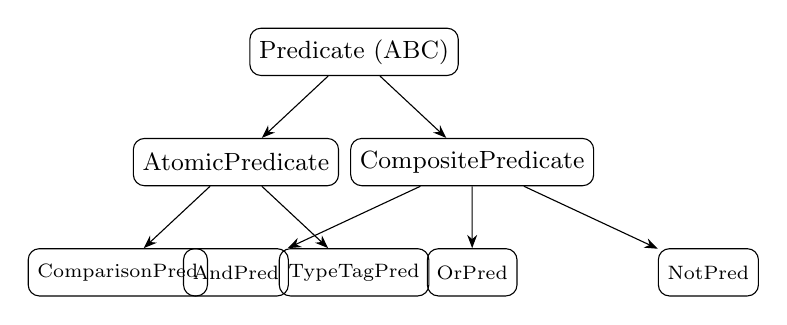
\begin{tikzpicture}[
  every node/.style={draw, rounded corners, font=\small, minimum height=0.6cm},
  level distance=1.4cm, sibling distance=3cm,
  edge from parent/.style={draw, -Stealth}
]
  \node {Predicate (ABC)}
    child { node {AtomicPredicate}
      child { node[font=\scriptsize] {ComparisonPred} }
      child { node[font=\scriptsize] {TypeTagPred} }
    }
    child { node {CompositePredicate}
      child { node[font=\scriptsize] {AndPred} }
      child { node[font=\scriptsize] {OrPred} }
      child { node[font=\scriptsize] {NotPred} }
    };
\end{tikzpicture}
\end{center}

Every predicate supports: \texttt{free\_vars()}, \texttt{substitute\_var()}, \texttt{negate()}.

These are the ``values'' that sections carry. Agreement between sections is checked by comparing their predicates via SMT.
\end{frame}

% ── SLIDE 55 ─────────────────────────────────────────────────
\begin{frame}{The Observation Site Category $\mathbf{S}$}
\textbf{Formally:} Deppy works with a \emph{category} $\mathbf{S}$ of observation sites.

\begin{description}
  \item[Objects] Sites (the 14 families)
  \item[Morphisms] Restriction maps (inclusion of one site's scope into another's)
  \item[Composition] Restriction is transitive
  \item[Identity] Every site restricts to itself
\end{description}

\vspace{0.3em}
The \textbf{semantic presheaf} is a functor $\Sem : \mathbf{S}^{\op} \to \Poset$:
\begin{itemize}
  \item To each site, assign its set of possible sections (ordered by information)
  \item To each morphism, assign a restriction function
\end{itemize}

This is where category theory enters. Let's build up to it properly.
\end{frame}

% ── SLIDE 56 ─────────────────────────────────────────────────
\begin{frame}{What You Need from PL for the Presentation}
\begin{enumerate}
  \item \textbf{Slide 3} mentions abstract interpretation + widening + precision loss.\\
        $\to$ You now know why: global fixpoint, $\mathcal{O}(|D|^k)$, widening overshoots.
  \item \textbf{Slide 4} claims $\rk H^1$ = minimum independent fixes.\\
        $\to$ You need sheaf theory for this. Coming in Part II--III.
  \item \textbf{Slide 5} claims exponential savings via decomposition.\\
        $\to$ $m \cdot d^{k/m} \ll d^k$. The ``sites'' are code regions.
  \item \textbf{Slide 7} mentions VCs and product covers.\\
        $\to$ Standard VC gen gives one big formula. Deppy factors it.
  \item \textbf{Slide 8} mentions $H^0$, $H^1$ certificates.\\
        $\to$ You need cohomology. Coming in Part III.
  \item \textbf{Slide 9} uses the Mayer-Vietoris exact sequence.\\
        $\to$ The crown jewel. Explained in Part III.
\end{enumerate}
\end{frame}

% ── SLIDES 57-60: Quick reference / transition ───────────────
\begin{frame}{PL Glossary for Quick Reference}
\footnotesize
\renewcommand{\arraystretch}{1.2}
\begin{tabular}{@{}lp{9cm}@{}}
\toprule
\textbf{Term} & \textbf{One-line definition} \\
\midrule
Abstract interpretation & Over-approximate program behavior on an abstract domain \\
Galois connection & Soundness link between concrete and abstract domains \\
Widening & Force convergence of ascending chains (loses precision) \\
Refinement type & Base type + logical predicate: $\{x:\tau \mid \varphi\}$ \\
Dependent type & Type that depends on a value: $\Pi_{n:\mathbb{N}} \texttt{Vec}(n)$ \\
Verification condition & Logical formula whose validity $\Rightarrow$ program correctness \\
SMT solver & Decision procedure for satisfiability in combined theories \\
CEGAR & Iterative refinement of abstractions using counterexamples \\
Bisimulation & Stepwise behavioral equivalence relation \\
SSA & Static single assignment: each variable assigned once \\
\bottomrule
\end{tabular}
\end{frame}

\begin{frame}{PL Glossary (cont.)}
\footnotesize
\renewcommand{\arraystretch}{1.2}
\begin{tabular}{@{}lp{9cm}@{}}
\toprule
\textbf{Term} & \textbf{One-line definition} \\
\midrule
Knuth-Bendix & Complete equational theories into confluent rewrite systems \\
Nelson-Oppen & Combine decision procedures for disjoint-signature theories \\
Separation logic & Reason about disjoint heap regions via $*$ connective \\
Frame rule & Local changes don't affect disjoint state \\
Type soundness & Well-typed programs don't get stuck \\
Curry-Howard & Proofs = programs, propositions = types \\
Predicate abstraction & Track boolean vector of predicate truth values \\
Fixpoint & Invariant solution of transfer-function iteration \\
Weakest precondition & Most permissive precondition ensuring a postcondition \\
Proof certificate & Machine-checkable evidence of validity \\
\bottomrule
\end{tabular}
\end{frame}

\begin{frame}{PL Notation Reference}
\begin{align*}
\Gamma \vdash e : \tau &\quad\text{Expression $e$ has type $\tau$ in context $\Gamma$} \\
\{x:\tau \mid \varphi\} &\quad\text{Refinement type: $\tau$ constrained by $\varphi$} \\
\Pi_{x:A} B(x) &\quad\text{Dependent function type} \\
\Sigma_{x:A} B(x) &\quad\text{Dependent pair type} \\
\mathrm{Id}_A(a,b) &\quad\text{Identity/equality type in $A$} \\
\alpha, \gamma &\quad\text{Abstraction and concretization (Galois connection)} \\
\nabla &\quad\text{Widening operator} \\
\text{wp}(c, Q) &\quad\text{Weakest precondition of $c$ for postcondition $Q$} \\
\sqsubseteq, \sqcup, \sqcap &\quad\text{Partial order, join, meet in a lattice}
\end{align*}
\end{frame}

% ╔═══════════════════════════════════════════════════════════════════════════╗
% ║  PART II: SHEAF THEORY (Slides 61-120)                                  ║
% ╚═══════════════════════════════════════════════════════════════════════════╝

\begin{frame}[plain]
\begin{center}
\vspace{2cm}
{\Huge\textbf{Part II}}\\[0.3em]
{\Large Sheaf Theory}\\[1em]
{\normalsize Categories $\to$ Presheaves $\to$ Sheaves $\to$\\
 Grothendieck Topologies $\to$ Descent}
\end{center}
\end{frame}

% ── SLIDE 62: What is a Category? ────────────────────────────
\begin{frame}{What Is a Category?}
\begin{block}{Definition}
A \emph{category} $\mathbf{C}$ consists of:
\begin{itemize}
  \item A collection of \emph{objects} $\Ob(\mathbf{C})$
  \item For each pair of objects $A, B$: a set of \emph{morphisms} $\Hom(A, B)$
  \item Composition: $g \circ f : A \to C$ whenever $f : A \to B$ and $g : B \to C$
  \item Identity: $\id_A : A \to A$ for each object $A$
\end{itemize}
\end{block}

\textbf{Laws:}
\begin{enumerate}
  \item Associativity: $(h \circ g) \circ f = h \circ (g \circ f)$
  \item Identity: $f \circ \id_A = f = \id_B \circ f$
\end{enumerate}
\end{frame}

% ── SLIDE 63: Examples of Categories ─────────────────────────
\begin{frame}{Examples of Categories}
\renewcommand{\arraystretch}{1.4}
\begin{tabular}{@{}lll@{}}
\toprule
\textbf{Category} & \textbf{Objects} & \textbf{Morphisms} \\
\midrule
$\Set$ & Sets & Functions \\
$\Ab$ & Abelian groups & Group homomorphisms \\
$\mathbf{Top}$ & Topological spaces & Continuous maps \\
$\mathbf{Vect}_k$ & Vector spaces over $k$ & Linear maps \\
$\Poset$ & Posets & Order-preserving maps \\
$\Open(X)$ & Open sets of $X$ & Inclusions $U \hookrightarrow V$ \\
\bottomrule
\end{tabular}

\vspace{0.5em}
\textbf{For deppy:} $\mathbf{S}$ = the \emph{site category}, with:
\begin{itemize}
  \item Objects = observation sites (14 families)
  \item Morphisms = restriction/reindexing maps
\end{itemize}
\end{frame}

% ── SLIDE 64: Functors ──────────────────────────────────────
\begin{frame}{Functors}
\begin{block}{Definition}
A \emph{functor} $F : \mathbf{C} \to \mathbf{D}$ maps:
\begin{itemize}
  \item Objects: $A \mapsto F(A)$
  \item Morphisms: $(f: A \to B) \mapsto (F(f): F(A) \to F(B))$
\end{itemize}
preserving composition and identities:
$F(g \circ f) = F(g) \circ F(f)$, \quad $F(\id_A) = \id_{F(A)}$.
\end{block}

\vspace{0.3em}
\textbf{A presheaf is a functor} $\Fscr : \mathbf{C}^{\op} \to \Set$ (or $\to \Poset$).

The ``$\op$'' reverses arrows: if $U \hookrightarrow V$ in the site category, the presheaf gives a \emph{restriction} map $\Fscr(V) \to \Fscr(U)$ going the other way.
\end{frame}

% ── SLIDE 65: Opposite Category ──────────────────────────────
\begin{frame}{The Opposite Category $\mathbf{C}^{\op}$}
\textbf{Definition:} $\mathbf{C}^{\op}$ has the same objects as $\mathbf{C}$, but all morphisms reversed:
\[
\Hom_{\mathbf{C}^{\op}}(A, B) = \Hom_{\mathbf{C}}(B, A)
\]

\textbf{Why?} A presheaf $\Fscr : \mathbf{C}^{\op} \to \Set$ is a \emph{contravariant} functor on $\mathbf{C}$.

\vspace{0.3em}
\textbf{Intuition:}
\begin{itemize}
  \item In $\Open(X)$: $U \subseteq V$ gives inclusion $U \hookrightarrow V$
  \item A presheaf reverses this: $\Fscr(V) \to \Fscr(U)$ (restrict from bigger to smaller)
  \item Going to a \emph{smaller} open set = looking \emph{more locally}
\end{itemize}
\end{frame}

% ── SLIDE 66: Natural Transformations ────────────────────────
\begin{frame}[fragile]{Natural Transformations}
\begin{block}{Definition}
A \emph{natural transformation} $\eta : F \Rightarrow G$ between functors $F, G : \mathbf{C} \to \mathbf{D}$ assigns to each object $A$ a morphism $\eta_A : F(A) \to G(A)$ such that for every $f : A \to B$:
\[
\eta_B \circ F(f) = G(f) \circ \eta_A
\]
\end{block}

\begin{center}
\begin{tikzcd}
F(A) \arrow{r}{\eta_A} \arrow{d}{F(f)} & G(A) \arrow{d}{G(f)} \\
F(B) \arrow{r}{\eta_B} & G(B)
\end{tikzcd}
\end{center}

\textbf{For deppy:} A natural transformation between presheaves = a way to compare the ``type information'' assigned by two different analyses, site by site, consistently.
\end{frame}

% ── SLIDE 67: Topological Spaces ────────────────────────────
\begin{frame}{Topological Spaces: The Original Setting}
\begin{block}{Definition}
A \emph{topological space} $(X, \tau)$ is a set $X$ with a collection $\tau$ of ``open sets'' such that:
\begin{enumerate}
  \item $\emptyset, X \in \tau$
  \item Arbitrary unions of open sets are open
  \item Finite intersections of open sets are open
\end{enumerate}
\end{block}

\vspace{0.3em}
\textbf{Why topology?} Sheaf theory was born here.
\begin{itemize}
  \item $X$ = a geometric space (manifold, variety, scheme)
  \item Open sets = regions where we can make local observations
  \item Restriction: zoom in from a big region to a smaller one
\end{itemize}

\textbf{For deppy:} $X$ = the program. Open sets = code regions (sites). Topology = which regions overlap.
\end{frame}

% ── SLIDE 68: Open Covers ──────────────────────────────────
\begin{frame}{Open Covers}
\begin{block}{Definition}
An \emph{open cover} of $U \subseteq X$ is a collection $\{U_i\}_{i \in I}$ of open sets such that $U = \bigcup_{i \in I} U_i$.
\end{block}

\textbf{Example:} Cover the circle $S^1$ with two arcs:
\begin{itemize}
  \item $U_1$ = top half (plus overlap)
  \item $U_2$ = bottom half (plus overlap)
  \item $U_1 \cap U_2$ = two small arcs (left and right overlaps)
\end{itemize}

\vspace{0.3em}
\textbf{For deppy:}
\begin{itemize}
  \item Cover $=$ \texttt{Cover} object: \texttt{sites}, \texttt{morphisms}, \texttt{overlaps}
  \item Sites = code regions; overlaps = shared variables / control flow
  \item \texttt{cover\_builder.py} constructs covers from the CFG
\end{itemize}
\end{frame}

% ── SLIDE 69: Presheaves Defined ────────────────────────────
\begin{frame}{Presheaves: Local Data with Restriction}
\begin{block}{Definition}
A \emph{presheaf} on a topological space $X$ is a functor $\Fscr : \Open(X)^{\op} \to \Set$.

Concretely: for each open $U$, a set $\Fscr(U)$ (``sections over $U$''), and for each inclusion $U \subseteq V$, a \emph{restriction map} $\rho_{V,U} : \Fscr(V) \to \Fscr(U)$.
\end{block}

\textbf{Axioms:}
\begin{enumerate}
  \item $\rho_{U,U} = \id$ (restricting to yourself does nothing)
  \item $\rho_{V,U} \circ \rho_{W,V} = \rho_{W,U}$ (restriction is transitive)
\end{enumerate}

\textbf{Example:} $\Fscr(U) = \{\text{continuous functions } U \to \mathbb{R}\}$. Restriction = literal restriction of a function to a smaller domain.
\end{frame}

% ── SLIDE 70: Presheaf Examples ─────────────────────────────
\begin{frame}{Presheaf Examples}
\begin{enumerate}
  \item \textbf{Continuous functions}: $\Fscr(U) = C^0(U, \mathbb{R})$.
        Restriction: $f|_V$ for $V \subseteq U$.

  \item \textbf{Smooth functions}: $\Fscr(U) = C^\infty(U, \mathbb{R})$.

  \item \textbf{Holomorphic functions}: $\Fscr(U) = \Oscr(U)$ on a complex manifold.

  \item \textbf{Constant presheaf}: $\Fscr(U) = A$ for all $U$. Restriction = $\id$.

  \item \textbf{Locally constant functions}: $\Fscr(U) = \{f : U \to A \mid f \text{ locally constant}\}$.
\end{enumerate}

\vspace{0.5em}
\textbf{Deppy's presheaf:} $\Sem(U_i) = \{\text{possible type sections at site } U_i\}$, ordered by information content. Restriction = forgetting information about variables not in scope at the smaller site.
\end{frame}

% ── SLIDE 71: Sections ──────────────────────────────────────
\begin{frame}{Sections of a Presheaf}
\textbf{A section} $s \in \Fscr(U)$ is an element of the presheaf at open set $U$.

\textbf{Global section:} $s \in \Fscr(X)$ --- defined on the entire space.
\textbf{Local section:} $s \in \Fscr(U)$ --- defined on one open set.

\vspace{0.5em}
\textbf{Notation:} $\Gamma(U, \Fscr) = \Fscr(U)$.

$\Gamma(X, \Fscr)$ = space of global sections.

\vspace{0.5em}
\textbf{In deppy:}
\begin{itemize}
  \item \texttt{LocalSection} = section at one site
  \item \texttt{GlobalSection} = collection of compatible local sections
  \item The whole point: can we \emph{assemble} local sections into a global one?
\end{itemize}
\end{frame}

% ── SLIDE 72: The Sheaf Condition ───────────────────────────
\begin{frame}{The Sheaf Condition (Locality + Gluing)}
A presheaf $\Fscr$ is a \textbf{sheaf} if for every open cover $\{U_i\}$ of $U$:

\begin{block}{Locality (Separation)}
If $s, t \in \Fscr(U)$ satisfy $s|_{U_i} = t|_{U_i}$ for all $i$, then $s = t$.
\end{block}

\begin{block}{Gluing}
If sections $s_i \in \Fscr(U_i)$ satisfy $s_i|_{U_i \cap U_j} = s_j|_{U_i \cap U_j}$ for all $i, j$, then there exists $s \in \Fscr(U)$ with $s|_{U_i} = s_i$ for all $i$.
\end{block}

\vspace{0.3em}
\textbf{In one sentence:} Compatible local data can be uniquely assembled into global data.

\textbf{In deppy terms:} If all sites' type sections agree on overlaps, there's a unique consistent global typing.
\end{frame}

% ── SLIDE 73: Sheaf vs Presheaf ─────────────────────────────
\begin{frame}{Sheaf vs.\ Presheaf: What Can Go Wrong}
\textbf{A presheaf that is NOT a sheaf:}

$\Fscr(U) = \{\text{bounded functions } U \to \mathbb{R}\}$.

Take $U_1 = (0, 1)$, $U_2 = (1, 2)$, $U_3 = (2, 3)$, \ldots

Each $f_n$ bounded on $U_n$, but $\bigcup f_n$ may be unbounded on $\bigcup U_n$.

The local sections ``glue'' set-theoretically, but the global function isn't in $\Fscr(\bigcup U_n)$.

\vspace{0.5em}
\textbf{Why this matters for PL:}
\begin{itemize}
  \item Local type assignments might be individually consistent\ldots
  \item \ldots but fail to glue globally (e.g., contradictory types at overlaps)
  \item The failure to glue is precisely an \textbf{obstruction}: a nontrivial $H^1$ class
\end{itemize}
\end{frame}

% ── SLIDE 74: Sheaves as an Equalizer ───────────────────────
\begin{frame}{Sheaves as an Equalizer}
The sheaf condition can be stated as an \emph{exact sequence}:
\[
0 \to \Fscr(U) \xrightarrow{\;\;\text{res}\;\;}
\prod_i \Fscr(U_i) \;\;
\substack{\xrightarrow{\;\;p\;\;} \\ \xrightarrow{\;\;q\;\;}}
\;\; \prod_{i < j} \Fscr(U_i \cap U_j)
\]

where $p$ and $q$ restrict from different sides of the overlap.

\vspace{0.3em}
\textbf{Meaning:}
\begin{itemize}
  \item $\Fscr(U)$ is the \emph{equalizer} of $p$ and $q$
  \item A global section = a tuple of local sections where both restriction paths agree
  \item This is the ``kernel'' of the difference map $p - q$
\end{itemize}

\textbf{This exact sequence is the beginning of the \v{C}ech complex} (Part III).
\end{frame}

% ── SLIDE 75: Stalks ────────────────────────────────────────
\begin{frame}{Stalks: The Infinitely Local View}
\begin{block}{Definition}
The \emph{stalk} of $\Fscr$ at a point $x \in X$ is:
\[
\Fscr_x = \varinjlim_{U \ni x} \Fscr(U) = \{(U, s) \mid x \in U, s \in \Fscr(U)\} / {\sim}
\]
where $(U, s) \sim (V, t)$ if $s|_W = t|_W$ for some $W \subseteq U \cap V$ with $x \in W$.
\end{block}

\textbf{Intuition:} The stalk is the ``germ'' of all sections at $x$. Two sections that agree near $x$ are identified.

\vspace{0.3em}
\textbf{In deppy:} \texttt{stalk.py} computes stalks for the equivalence checker.
The stalk at a program point = the ``ultimate local type'' considering all surrounding contexts.

\vspace{0.3em}
\textbf{Key property:} A morphism of sheaves is an isomorphism iff it's an isomorphism on all stalks.
\end{frame}

% ── SLIDE 76: Restriction Maps Concretely ───────────────────
\begin{frame}[fragile]{Restriction Maps in Deppy}
\begin{lstlisting}
@dataclass(frozen=True)
class ConcreteMorphism:
    _source: SiteId    # larger site
    _target: SiteId    # smaller site
    projection: Optional[Dict[str, str]] = None

    def restrict(self, section: LocalSection) -> LocalSection:
        """Restrict section from source to target."""
        # Keep only the refinements relevant to the target
        if self.projection:
            new_refs = {k: section.refinements[v]
                        for k, v in self.projection.items()
                        if v in section.refinements}
        else:
            new_refs = dict(section.refinements)
        return LocalSection(
            site_id=self._target,
            carrier_type=section.carrier_type,
            refinements=new_refs,
            trust=section.trust,
        )
\end{lstlisting}

Restriction = project out irrelevant variables. Exactly like the math.
\end{frame}

% ── SLIDE 77: Sheafification ────────────────────────────────
\begin{frame}{Sheafification: Turning Presheaves into Sheaves}
\textbf{Not every presheaf is a sheaf.} But there's a universal fix:

\begin{block}{Sheafification}
For any presheaf $\Fscr$, there exists a sheaf $\Fscr^+$ and a map $\theta : \Fscr \to \Fscr^+$ such that:
\begin{enumerate}
  \item $\theta$ preserves stalks: $\Fscr_x \cong \Fscr^+_x$ for all $x$
  \item $\theta$ is universal: any map from $\Fscr$ to a sheaf factors through $\Fscr^+$
\end{enumerate}
\end{block}

\textbf{Construction:} Two rounds of the ``\'etal\'e space'' construction (plus construction).

\vspace{0.3em}
\textbf{For deppy:} The initial local inference gives a presheaf. The gluing check + $H^1$ computation is essentially asking: \emph{how far is this presheaf from being a sheaf?} The obstructions measure the failure.
\end{frame}

% ── SLIDE 78: Morphisms of Sheaves ──────────────────────────
\begin{frame}{Morphisms of Sheaves}
\begin{block}{Definition}
A \emph{morphism} of sheaves $\varphi : \Fscr \to \Gscr$ is a natural transformation: for each $U$, a map $\varphi_U : \Fscr(U) \to \Gscr(U)$ compatible with restrictions.
\end{block}

\vspace{0.3em}
\textbf{In deppy:} \texttt{sheaf\_morphism.py} defines maps between presheaves.

Used for:
\begin{itemize}
  \item \textbf{Equivalence checking}: Is there an isomorphism $\Sem_f \cong \Sem_g$?
  \item \textbf{Refinement checking}: Is there a monomorphism $\text{Spec} \hookrightarrow \Sem_f$?
  \item \textbf{Proof transport}: Transporting proofs from one site to another
\end{itemize}

\textbf{Key:} Isomorphisms can be checked stalk-by-stalk (a local property).
\end{frame}

% ── SLIDE 79: Espace Étalé ─────────────────────────────────
\begin{frame}{The \'Etal\'e Space (Intuition)}
\textbf{Alternative view of a sheaf:} Instead of assigning sets to opens, build a space:

\[
\text{\'Et}(\Fscr) = \coprod_{x \in X} \Fscr_x \quad\text{(disjoint union of all stalks)}
\]

with a natural projection $\pi : \text{\'Et}(\Fscr) \to X$.

\textbf{Sections of the \'etal\'e space} = sections of the sheaf.

\vspace{0.5em}
\textbf{Intuition:} Picture a ``field'' over $X$ where at each point there's a fiber (the stalk). A section is a continuous choice of one element from each fiber.

\textbf{For deppy:} Think of each program point having a ``fiber'' of possible type assignments. A global section picks one assignment per point, consistently.
\end{frame}

% ── SLIDE 80: Grothendieck Topologies ───────────────────────
\begin{frame}{Beyond Topological Spaces: Grothendieck Topologies}
\textbf{Problem:} Not everything has a classical topology (e.g., algebraic geometry, PL).

\textbf{Solution:} Grothendieck generalized ``open cover'' to work on \emph{any} category.

\begin{block}{Grothendieck Topology (simplified)}
A \emph{Grothendieck topology} on a category $\mathbf{C}$ assigns to each object $U$ a collection of \emph{covering families} $\{U_i \to U\}$ satisfying:
\begin{enumerate}
  \item \textbf{Identity}: $\{\id : U \to U\}$ is a cover
  \item \textbf{Stability}: Covers pull back: if $\{U_i \to U\}$ covers and $V \to U$, then $\{U_i \times_U V \to V\}$ covers
  \item \textbf{Transitivity}: Covers of covers are covers
\end{enumerate}
\end{block}
\end{frame}

% ── SLIDE 81: Sites ─────────────────────────────────────────
\begin{frame}{Sites = Category + Grothendieck Topology}
\begin{block}{Definition}
A \emph{site} is a pair $(\mathbf{C}, J)$ where $\mathbf{C}$ is a category and $J$ is a Grothendieck topology on $\mathbf{C}$.
\end{block}

A \textbf{sheaf on a site} $(\mathbf{C}, J)$ is a presheaf $\Fscr : \mathbf{C}^{\op} \to \Set$ satisfying the sheaf condition for every $J$-cover.

\vspace{0.5em}
\textbf{In deppy:}
\begin{itemize}
  \item $\mathbf{C} = \mathbf{S}$ (site category of 14 families)
  \item $J$ = determined by the cover builder (which overlaps are ``real'')
  \item The \texttt{GrothendieckTopology} protocol enforces the three axioms
  \item Sheaf condition checked by \texttt{section\_gluing.py}
\end{itemize}

This is the most general setting. It works for programs because programs don't have a classical topology---but they do have a site category.
\end{frame}

% ── SLIDE 82: Why Grothendieck for Programs ─────────────────
\begin{frame}{Why Programs Need Grothendieck Topologies}
\textbf{Classical topology fails for programs:}
\begin{itemize}
  \item No meaningful metric on code
  \item ``Open sets'' of program points aren't literally open
  \item Overlaps are syntactic (shared variables), not geometric
\end{itemize}

\textbf{Grothendieck topology works:}
\begin{itemize}
  \item Objects = code regions (any granularity)
  \item Morphisms = inclusions (this region is part of that one)
  \item Covers = ``enough regions to see everything''
  \item The axioms are about \emph{composability}, not geometry
\end{itemize}

\vspace{0.3em}
The observation site category $\mathbf{S}$ with its covering families is a genuine site in the Grothendieck sense. This is what makes the cohomological machinery applicable.
\end{frame}

% ── SLIDE 83: The Category Open(X) ─────────────────────────
\begin{frame}{Example: $\Open(X)$ as a Site}
For a topological space $X$:
\begin{itemize}
  \item \textbf{Category}: $\Open(X)$ --- objects are open sets, morphisms are inclusions
  \item \textbf{Topology}: A family $\{U_i \hookrightarrow U\}$ covers iff $\bigcup U_i = U$
  \item \textbf{Sheaf}: The usual notion from topology
\end{itemize}

\textbf{Key properties:}
\begin{itemize}
  \item Every inclusion $U_i \hookrightarrow U$ is a monomorphism
  \item Fiber products exist: $U_i \times_U U_j = U_i \cap U_j$
  \item The nerve of the cover gives the \v{C}ech complex
\end{itemize}

\vspace{0.3em}
Deppy's site category has all these properties (by construction).
\end{frame}

% ── SLIDE 84: Fiber Products / Pullbacks ────────────────────
\begin{frame}[fragile]{Fiber Products (Pullbacks)}
\begin{block}{Definition}
The \emph{fiber product} $A \times_C B$ is the universal object making the square commute:
\end{block}

\begin{center}
\begin{tikzcd}
A \times_C B \arrow{r} \arrow{d} & B \arrow{d}{g} \\
A \arrow{r}{f} & C
\end{tikzcd}
\end{center}

\textbf{In $\Open(X)$:} $U_i \times_U U_j = U_i \cap U_j$ (intersection).

\textbf{In deppy:} \texttt{fiber\_product.py} computes the ``overlap'' between two sites:
\begin{itemize}
  \item Shared variables
  \item Shared control-flow paths
  \item The intersection of their scopes
\end{itemize}

This is used in the equivalence checker to compute transition functions on overlaps.
\end{frame}

% ── SLIDE 85: Descent Data ──────────────────────────────────
\begin{frame}{Descent Data}
\begin{block}{Definition}
\emph{Descent data} for a cover $\{U_i \to U\}$ of an object in a sheaf consists of:
\begin{enumerate}
  \item \textbf{Local objects}: sections $s_i \in \Fscr(U_i)$
  \item \textbf{Transition maps}: isomorphisms $\varphi_{ij} : s_i|_{U_{ij}} \xrightarrow{\sim} s_j|_{U_{ij}}$
  \item \textbf{Cocycle condition}: $\varphi_{jk} \circ \varphi_{ij} = \varphi_{ik}$ on triple overlaps
\end{enumerate}
\end{block}

\textbf{Descent} holds if every descent datum comes from a global object.

\vspace{0.3em}
\textbf{In deppy:}
\begin{itemize}
  \item Local objects = local sections at each site
  \item Transition maps = how sections at adjacent sites relate
  \item Cocycle condition = checked by \texttt{cohomology.py}
  \item Descent holds iff $H^1 = 0$
\end{itemize}
\end{frame}

% ── SLIDE 86: Descent = Effective Epimorphism ───────────────
\begin{frame}{When Descent Holds}
\textbf{Descent holds} (= the cover is an ``effective epimorphism'') when:

\[
\Fscr(U) \xrightarrow{\;\sim\;} \text{DescentData}(\{U_i \to U\}, \Fscr)
\]

\textbf{Meaning:} Specifying a global section is \emph{equivalent} to specifying compatible local sections.

\vspace{0.5em}
\textbf{When descent fails:}
\begin{itemize}
  \item The local sections don't extend to a global one
  \item The obstruction lives in $H^1$ (first cohomology)
  \item Deppy reports this as: ``these sites have incompatible type assignments''
\end{itemize}

\vspace{0.3em}
\textbf{For PL:} Descent failure = type error. Descent success = well-typed program (relative to the cover).
\end{frame}

% ── SLIDE 87: The Nerve of a Cover ──────────────────────────
\begin{frame}{The Nerve of a Cover}
\begin{block}{Definition}
The \emph{nerve} $N(\Uscr)$ of a cover $\Uscr = \{U_i\}$ is a simplicial complex:
\begin{itemize}
  \item 0-simplices: $U_i$ (the sites)
  \item 1-simplices: $U_i \cap U_j \neq \emptyset$ (pairwise overlaps)
  \item 2-simplices: $U_i \cap U_j \cap U_k \neq \emptyset$ (triple overlaps)
  \item $\vdots$
\end{itemize}
\end{block}

\textbf{The nerve captures the combinatorial structure of the cover.}

In deppy: \texttt{Cover.overlaps} = the 1-skeleton of the nerve. Triple overlaps are computed on demand by the cohomology module.

\vspace{0.3em}
The \v{C}ech cohomology is computed from this nerve.
\end{frame}

% ── SLIDE 88: Example: Covering a Function ──────────────────
\begin{frame}[fragile]{Example: Covering a Python Function}
\begin{lstlisting}
def f(x: int, y: int) -> int:
    if x > 0:          # site U1 (branch guard)
        z = x + y      # site U2 (SSA value)
    else:
        z = x - y      # site U3 (SSA value)
    return z / y       # site U4 (error site: y=0?)
\end{lstlisting}

\textbf{Cover:}
\begin{itemize}
  \item $U_1$: branch guard ($x > 0$)
  \item $U_2$: true branch ($z = x + y$, inherits $x > 0$)
  \item $U_3$: false branch ($z = x - y$, inherits $x \leq 0$)
  \item $U_4$: return site ($z / y$)
  \item Overlaps: $(U_1, U_2)$, $(U_1, U_3)$, $(U_2, U_4)$, $(U_3, U_4)$
\end{itemize}

\textbf{Obstruction:} At overlap $(U_2, U_4)$ and $(U_3, U_4)$: site $U_4$ requires $y \neq 0$, but neither $U_2$ nor $U_3$ guarantees it.
\end{frame}

% ── SLIDE 89: The Sheaf of Type Sections ────────────────────
\begin{frame}{The Semantic Presheaf $\Sem$}
\textbf{Deppy's presheaf:}
\[
\Sem : \mathbf{S}^{\op} \to \Poset
\]

\begin{itemize}
  \item $\Sem(U_i) = \{\text{possible type sections at site } U_i\}$
  \item Ordered by \emph{information content}: $s \sqsubseteq t$ if $t$ knows everything $s$ does and more
  \item Restriction: $\Sem(f)(s) = s|_{\text{smaller site}}$ (forget irrelevant variables)
\end{itemize}

\vspace{0.3em}
\textbf{Sections carry:}
\begin{enumerate}
  \item Carrier type (int, str, List[int], \ldots)
  \item Refinement predicates ($x > 0$, $\texttt{len}(a) = n$, \ldots)
  \item Trust level (proof-backed, trace-backed, assumed, \ldots)
  \item Witnesses (proof terms, test cases, \ldots)
\end{enumerate}
\end{frame}

% ── SLIDE 90: The Information Order ─────────────────────────
\begin{frame}{The Information Order on Sections}
\textbf{Protocol:} \texttt{InformationOrder} --- defines when one section is ``more informative'' than another.

\[
s_1 \sqsubseteq s_2 \;\;\text{iff}\;\; \text{refinements}(s_1) \subseteq \text{refinements}(s_2) \;\wedge\; \text{trust}(s_1) \leq \text{trust}(s_2)
\]

\textbf{This makes $\Sem(U_i)$ a poset.}

\vspace{0.3em}
\textbf{Why ordered?}
\begin{itemize}
  \item The presheaf takes values in $\Poset$, not just $\Set$
  \item This lets us talk about ``more precise'' vs ``less precise'' sections
  \item The fixpoint computation (forward/backward synthesis) ascends this order
  \item Join = merge compatible information; meet = take common knowledge
\end{itemize}
\end{frame}

% ── SLIDE 91: The Sheaf Condition for Programs ──────────────
\begin{frame}{The Sheaf Condition for Programs}
\textbf{Does $\Sem$ satisfy the sheaf condition?}

\textbf{Locality:} If two global typings agree at every site, they're the same. \yes

\textbf{Gluing:} If local sections agree on all overlaps, a global section exists. \textcolor{meh}{Sometimes.}

\vspace{0.5em}
\textbf{When gluing fails:}
\begin{itemize}
  \item There's a genuine type error (bug)
  \item Or the cover is too coarse (need more sites)
  \item Or the local inference was imprecise
\end{itemize}

\textbf{Deppy's approach:} Don't require $\Sem$ to be a sheaf. Instead, \emph{measure} the failure via $H^1$. The obstructions tell you exactly where and how gluing fails.
\end{frame}

% ── SLIDE 92: Sheaves of Modules and Abelian Sheaves ────────
\begin{frame}{Sheaves of Abelian Groups}
For cohomology, we need \emph{algebraic} structure on our sheaves.

\textbf{A sheaf of abelian groups}: $\Fscr : \Open(X)^{\op} \to \Ab$.
\begin{itemize}
  \item Each $\Fscr(U)$ is an abelian group
  \item Restriction maps are group homomorphisms
  \item Sheaf condition holds as before
\end{itemize}

\textbf{In deppy:} The cohomology computations work over $\mathbb{F}_2 = \{0, 1\}$:
\begin{itemize}
  \item Each overlap is either ``agrees'' (0) or ``disagrees'' (1)
  \item The coboundary matrix has entries in $\mathbb{F}_2$
  \item $H^1$ is a vector space over $\mathbb{F}_2$
  \item $\dim H^1$ = number of independent obstructions
\end{itemize}
\end{frame}

% ── SLIDE 93: Short Exact Sequences of Sheaves ──────────────
\begin{frame}{Short Exact Sequences}
\begin{block}{Definition}
A sequence $0 \to \Fscr' \xrightarrow{\alpha} \Fscr \xrightarrow{\beta} \Fscr'' \to 0$ is \emph{exact} if:
\begin{itemize}
  \item $\alpha$ is injective (monomorphism)
  \item $\beta$ is surjective (epimorphism)
  \item $\ker(\beta) = \im(\alpha)$
\end{itemize}
\end{block}

\textbf{For sheaves:} Exactness is checked \emph{stalkwise} (local property).

A short exact sequence of sheaves may \emph{fail} to give a short exact sequence on global sections. The obstruction to surjectivity on global sections is measured by $H^1(\Fscr')$.

\vspace{0.3em}
\textbf{This is the origin of sheaf cohomology:} it measures the failure of ``local surjectivity $\Rightarrow$ global surjectivity.''
\end{frame}

% ── SLIDE 94: The Global Sections Functor ───────────────────
\begin{frame}{The Global Sections Functor $\Gamma$}
\textbf{Definition:} $\Gamma(X, -) : \mathbf{Sh}(X) \to \Ab$ sends $\Fscr \mapsto \Fscr(X)$.

$\Gamma$ is \emph{left exact}: it preserves exact sequences on the left:
\[
0 \to \Gamma(\Fscr') \to \Gamma(\Fscr) \to \Gamma(\Fscr'')
\]
but the last map may not be surjective.

\vspace{0.3em}
\textbf{Sheaf cohomology} $H^n(X, \Fscr)$ = the \emph{right derived functors} of $\Gamma$.

$H^0(X, \Fscr) = \Gamma(X, \Fscr)$ (global sections).

$H^1(X, \Fscr)$ = first obstruction to extending local data globally.

\vspace{0.3em}
\textbf{For deppy:} $H^0$ = the global typing (if it exists). $H^1$ = obstructions to global typing.
\end{frame}

% ── SLIDE 95: Recap: The Mathematical Dictionary ────────────
\begin{frame}{The Mathematical Dictionary}
\begin{center}
\renewcommand{\arraystretch}{1.4}
\footnotesize
\begin{tabular}{@{}ll@{}}
\toprule
\textbf{Math} & \textbf{Deppy} \\
\midrule
Topological space $X$ & Program \\
Open set $U_i$ & Observation site (code region) \\
Open cover $\{U_i\}$ & \texttt{Cover} (sites + overlaps) \\
Presheaf $\Fscr$ & \texttt{ConcretePresheaf} (type info per site) \\
Section $s \in \Fscr(U)$ & \texttt{LocalSection} (type at one site) \\
Global section $s \in \Fscr(X)$ & \texttt{GlobalSection} (consistent global typing) \\
Restriction $s|_V$ & \texttt{ConcreteMorphism.restrict()} \\
Gluing condition & \texttt{check\_gluing\_condition()} \\
Stalk $\Fscr_x$ & Ultimate local type at a point \\
Descent data & Local sections + transition maps + cocycle \\
$H^0 = 0$ & No global section (disconnected cover) \\
$H^1 = 0$ & Gluing succeeds (no type errors) \\
$H^1 \neq 0$ & Obstructions (type errors) \\
\bottomrule
\end{tabular}
\end{center}
\end{frame}

% ── SLIDE 96: The Coefficient Sheaf for Equivalence ─────────
\begin{frame}{The Coefficient Sheaf $\Iso(\Sem_f, \Sem_g)$}
For equivalence checking, the coefficient sheaf is:
\[
\Iso(\Sem_f, \Sem_g)(U_i) = \{\text{isomorphisms } \Sem_f(U_i) \xrightarrow{\sim} \Sem_g(U_i)\}
\]

\textbf{This is the sheaf of \emph{local equivalences}.}

\begin{itemize}
  \item If $\Iso(\Sem_f, \Sem_g)(U_i)$ is nonempty: $f$ and $g$ behave the same on $U_i$
  \item If nonempty for all $i$: they're locally equivalent everywhere
  \item The question: do these local equivalences \emph{glue}?
\end{itemize}

\textbf{Cohomology answers:}
\begin{itemize}
  \item $H^0(\Iso) \neq 0$ $\Rightarrow$ there is a global isomorphism
  \item $H^1(\Iso) = 0$ $\Rightarrow$ local isomorphisms glue to global
  \item $H^1(\Iso) \neq 0$ $\Rightarrow$ obstruction to global equivalence
\end{itemize}
\end{frame}

% ── SLIDE 97: Transition Functions ──────────────────────────
\begin{frame}{Transition Functions}
Given local isomorphisms $\eta_i : \Sem_f(U_i) \xrightarrow{\sim} \Sem_g(U_i)$, the \textbf{transition functions} on overlaps are:
\[
g_{ij} = \eta_j|_{U_{ij}} \circ (\eta_i|_{U_{ij}})^{-1} : \Sem_f(U_{ij}) \to \Sem_f(U_{ij})
\]

\textbf{These form a \v{C}ech 1-cocycle} in $C^1(\Uscr, \Iso)$.

\vspace{0.3em}
\textbf{Cocycle condition} on triple overlaps:
\[
g_{ij} \circ g_{jk} = g_{ik} \quad\text{on } U_i \cap U_j \cap U_k
\]

\textbf{In deppy:} \texttt{descent.py} builds these transition functions from local equivalence judgments. \texttt{cohomology.py} checks the cocycle condition via SMT.
\end{frame}

% ── SLIDE 98: Vector Bundles Analogy ────────────────────────
\begin{frame}{Analogy: Vector Bundles}
\textbf{A vector bundle} over $X$:
\begin{itemize}
  \item Local trivialization on each $U_i$: $E|_{U_i} \cong U_i \times \mathbb{R}^n$
  \item Transition functions: $g_{ij} : U_{ij} \to GL(n, \mathbb{R})$
  \item Cocycle: $g_{ij} g_{jk} = g_{ik}$ on $U_{ijk}$
  \item Classified by $H^1(X, GL(n))$
\end{itemize}

\textbf{Deppy's equivalence checker is the same pattern:}
\begin{itemize}
  \item Local equivalence on each site: $\Sem_f(U_i) \cong \Sem_g(U_i)$
  \item Transition functions: $g_{ij}$ from composing local isomorphisms
  \item Cocycle condition: checked by \texttt{cohomology.py}
  \item Classified by $H^1(\Uscr, \Iso(\Sem_f, \Sem_g))$
\end{itemize}
\end{frame}

% ── SLIDE 99: Effective Descent ─────────────────────────────
\begin{frame}{Effective Descent}
\begin{block}{Theorem (Effective Descent)}
Local equivalences $\{\eta_i : \Sem_f(U_i) \xrightarrow{\sim} \Sem_g(U_i)\}$ glue to a \emph{global} equivalence if and only if $H^1(\Uscr, \Iso(\Sem_f, \Sem_g)) = 0$.
\end{block}

\textbf{This is the central theorem of deppy's equivalence checker.}

\vspace{0.3em}
\textbf{Comparison with standard modular checking:}
\begin{itemize}
  \item Standard: ``interfaces match $\Rightarrow$ equivalent'' --- \emph{sound but not complete}
  \item Sheaf: ``$H^1 = 0 \Leftrightarrow$ globally equivalent'' --- \emph{sound AND complete} for the cover
\end{itemize}

\vspace{0.3em}
The completeness direction is the key upgrade. Standard tools can reject equivalent programs; the sheaf approach doesn't.
\end{frame}

% ── SLIDE 100: Topos Theory (Brief Mention) ─────────────────
\begin{frame}{Topos Theory (One Slide)}
\textbf{A topos} is a category that ``behaves like $\Set$'':
\begin{itemize}
  \item Has finite limits and colimits
  \item Has exponential objects (function spaces)
  \item Has a subobject classifier $\Omega$ (generalized truth values)
\end{itemize}

\textbf{The category $\mathbf{Sh}(\mathbf{C}, J)$} of sheaves on a site is a \emph{Grothendieck topos}.

\vspace{0.3em}
\textbf{For deppy:} \texttt{topos.py} in the equivalence module. The topos structure gives:
\begin{itemize}
  \item Internal logic for reasoning about ``local truth''
  \item $\Omega(U) = \{\text{cribles on } U\}$ = ``how true is this at $U$?''
  \item But you don't need topos theory for the presentation---just know it's there
\end{itemize}
\end{frame}

% ── SLIDES 101-110: More sheaf theory details ────────────────

\begin{frame}{Sheaves on the Zariski Site (Motivation)}
\textbf{Historical context:} Sheaves were developed for algebraic geometry.

\textbf{The Zariski topology} on $\text{Spec}(R)$:
\begin{itemize}
  \item Points = prime ideals of a ring $R$
  \item Open sets = complements of $V(I) = \{\mathfrak{p} \supseteq I\}$
  \item The structure sheaf $\Oscr_X$ assigns to each open the localization
\end{itemize}

\textbf{Why mention this?} The pattern is:
\begin{enumerate}
  \item Define a ``space'' (Spec, program, \ldots)
  \item Cover it with local patches
  \item Put a sheaf on it (structure sheaf, type presheaf, \ldots)
  \item Use cohomology to understand global behavior from local data
\end{enumerate}

Deppy follows this exact pattern, just with programs instead of rings.
\end{frame}

\begin{frame}{Refinement: Covers Can Be Refined}
\begin{block}{Definition}
A cover $\mathcal{V} = \{V_j\}$ \emph{refines} $\Uscr = \{U_i\}$ if there exists a map $\tau : J \to I$ with $V_j \subseteq U_{\tau(j)}$ for all $j$.
\end{block}

\textbf{Property:} \v{C}ech cohomology is stable under refinement. More precisely:
\[
\check{H}^n(\Uscr, \Fscr) \to \check{H}^n(\mathcal{V}, \Fscr) \quad\text{(restriction map)}
\]
and the direct limit over all covers gives the ``true'' \v{C}ech cohomology.

\vspace{0.3em}
\textbf{For deppy:} If a cover is too coarse (false positive obstructions), refine it by adding more sites. The obstructions can only decrease.
\end{frame}

\begin{frame}{The Leray Spectral Sequence (Just the Idea)}
\textbf{When covers are ``good enough'':}

\begin{block}{Leray's Theorem}
If the cover $\Uscr$ is ``acyclic'' ($H^q(U_{i_0 \cdots i_p}, \Fscr) = 0$ for $q > 0$), then \v{C}ech cohomology equals sheaf cohomology:
\[
\check{H}^n(\Uscr, \Fscr) \cong H^n(X, \Fscr)
\]
\end{block}

\textbf{In practice:} Good covers (where all intersections are ``contractible'') give exact results.

\textbf{For deppy:} The covers from the CFG are ``good'' in this sense---each site is a convex code region. So the \v{C}ech computation gives the right answer.
\end{frame}

\begin{frame}{Sheaves of Rings and Modules}
\textbf{Enriched structure:}
\begin{itemize}
  \item A \emph{sheaf of rings} $\Oscr_X$: each $\Oscr_X(U)$ is a ring
  \item A \emph{sheaf of modules} over $\Oscr_X$: each $\Fscr(U)$ is an $\Oscr_X(U)$-module
  \item Restriction maps are ring/module homomorphisms
\end{itemize}

\vspace{0.3em}
\textbf{For deppy:}
\begin{itemize}
  \item The ``ring'' is the algebra of predicates (conjunction = multiplication, disjunction = addition over $\mathbb{F}_2$)
  \item Sections are ``modules'' over this ring
  \item This algebraic structure is what makes $H^1$ computations tractable: Gaussian elimination over $\mathbb{F}_2$
\end{itemize}
\end{frame}

\begin{frame}{Direct and Inverse Image Sheaves}
\textbf{Given a map} $f : X \to Y$:

\textbf{Direct image} (pushforward): $f_* \Fscr(V) = \Fscr(f^{-1}(V))$

\textbf{Inverse image} (pullback): $f^{-1}\Gscr(U) = \varinjlim_{V \supseteq f(U)} \Gscr(V)$

\vspace{0.5em}
\textbf{For deppy:}
\begin{itemize}
  \item Function call $f$ maps caller's sites to callee's sites
  \item \textbf{Pushforward}: transport section from callee back to caller
  \item \textbf{Pullback}: transport requirements from caller to callee
  \item \texttt{section\_transport.py} implements these operations
\end{itemize}

This is how interprocedural analysis works sheaf-theoretically.
\end{frame}

\begin{frame}{Adjunctions (Why Direct/Inverse Are Paired)}
\textbf{Fundamental adjunction:}
\[
\Hom_Y(f^{-1}\Gscr, \Fscr) \cong \Hom_X(\Gscr, f_*\Fscr)
\]

\textbf{$f^{-1}$ is left adjoint to $f_*$.}

\vspace{0.5em}
\textbf{What this means practically:}
\begin{itemize}
  \item Pulling back a spec from caller and pushing forward a proof from callee are ``dual'' operations
  \item The adjunction ensures they compose correctly
  \item This is why section transport preserves the sheaf condition
\end{itemize}

\vspace{0.3em}
\textbf{For the presentation:} You won't need adjunctions on stage. But knowing they're there explains \emph{why} the interprocedural analysis is sound.
\end{frame}

\begin{frame}{Locally Free Sheaves}
\begin{block}{Definition}
A sheaf $\Fscr$ is \emph{locally free of rank $n$} if each stalk $\Fscr_x \cong \Oscr_{X,x}^n$.
\end{block}

\textbf{Example:} The tangent bundle of a smooth manifold is a locally free sheaf.

\vspace{0.3em}
\textbf{For deppy:} The type sections at most sites look the same (same number of tracked variables, same refinement structure). This ``local uniformity'' is what makes the coboundary matrix well-defined and the Gaussian elimination tractable.

\vspace{0.3em}
If the sheaf were wildly non-uniform across sites, the $\mathbb{F}_2$ linear algebra trick wouldn't work.
\end{frame}

\begin{frame}{Support of a Sheaf}
\begin{block}{Definition}
The \emph{support} of a section $s \in \Fscr(U)$ is:
\[
\text{supp}(s) = \{x \in U \mid s_x \neq 0 \text{ in } \Fscr_x\}
\]
The support of the sheaf is $\text{supp}(\Fscr) = \{x \mid \Fscr_x \neq 0\}$.
\end{block}

\textbf{For deppy:}
\begin{itemize}
  \item Support of an obstruction = the program points where the type error manifests
  \item An obstruction with small support = localized bug
  \item An obstruction with large support = systemic design issue
  \item The \texttt{obstruction\_ranker.py} uses support size for severity ranking
\end{itemize}
\end{frame}

\begin{frame}{Flasque (Flabby) Sheaves}
\begin{block}{Definition}
A sheaf $\Fscr$ is \emph{flasque} if every restriction map $\Fscr(V) \to \Fscr(U)$ is surjective (every local section extends to a bigger open set).
\end{block}

\textbf{Key property:} Flasque sheaves have trivial cohomology: $H^n(\Fscr) = 0$ for $n > 0$.

\vspace{0.3em}
\textbf{For deppy:} If the type presheaf were flasque, there would be no obstructions---every local typing extends globally. This never happens for real programs (that would mean ``every program is well-typed'').

\vspace{0.3em}
Flasque sheaves are used in the \emph{Godement resolution} to compute cohomology. Deppy uses \v{C}ech cohomology instead (more computational).
\end{frame}

\begin{frame}{Summary: Sheaf Theory for the Presentation}
\textbf{What you need to confidently present:}

\begin{enumerate}
  \item A \textbf{presheaf} assigns data to each open set with compatible restrictions
  \item A \textbf{sheaf} satisfies gluing: compatible local data $\to$ unique global data
  \item \textbf{Grothendieck topology} generalizes ``open cover'' to any category
  \item A \textbf{site} = category + Grothendieck topology
  \item \textbf{Descent data} = local objects + transition functions + cocycle condition
  \item \textbf{Descent holds} iff $H^1 = 0$ (local sections glue globally)
  \item The \textbf{nerve} of a cover gives the combinatorial structure for \v{C}ech cohomology
  \item Deppy's \textbf{site category} $\mathbf{S}$ with 14 site families is a genuine Grothendieck site
\end{enumerate}
\end{frame}

% ── SLIDES 111-120: Sheaf glossary and notation ──────────────

\begin{frame}{Sheaf Theory Glossary}
\footnotesize
\renewcommand{\arraystretch}{1.2}
\begin{tabular}{@{}lp{8.5cm}@{}}
\toprule
\textbf{Term} & \textbf{One-line definition} \\
\midrule
Presheaf & Functor $\mathbf{C}^{\op} \to \Set$: data + restriction maps \\
Sheaf & Presheaf satisfying locality + gluing \\
Section & Element of $\Fscr(U)$; ``local data at $U$'' \\
Global section & Section over the whole space: $s \in \Fscr(X)$ \\
Stalk & Colimit of all sections at a point: $\Fscr_x = \varinjlim \Fscr(U)$ \\
Restriction & Map $\Fscr(V) \to \Fscr(U)$ for $U \subseteq V$ \\
Grothendieck topology & Axiomatic notion of ``covering family'' \\
Site & Category + Grothendieck topology \\
Descent data & Local objects + transition maps + cocycle condition \\
Nerve & Simplicial complex from a cover \\
\bottomrule
\end{tabular}
\end{frame}

\begin{frame}{Sheaf Theory Glossary (cont.)}
\footnotesize
\renewcommand{\arraystretch}{1.2}
\begin{tabular}{@{}lp{8.5cm}@{}}
\toprule
\textbf{Term} & \textbf{One-line definition} \\
\midrule
Sheafification & Universal way to turn a presheaf into a sheaf \\
\'Etal\'e space & Disjoint union of stalks with natural topology \\
Morphism of sheaves & Natural transformation compatible with restrictions \\
Direct image $f_*$ & Push a sheaf forward along a map \\
Inverse image $f^{-1}$ & Pull a sheaf back along a map \\
Locally free & Stalks are free modules of constant rank \\
Flasque & All restriction maps surjective \\
Support & Set of points where the sheaf/section is nonzero \\
Fiber product & Categorical intersection: $A \times_C B$ \\
Cover refinement & Finer cover that maps into a coarser one \\
\bottomrule
\end{tabular}
\end{frame}

\begin{frame}{Sheaf Notation Reference}
\begin{align*}
\Fscr(U) \;=\; \Gamma(U, \Fscr) &\quad\text{Sections of $\Fscr$ over $U$} \\
\rho_{V,U} : \Fscr(V) \to \Fscr(U) &\quad\text{Restriction map ($U \subseteq V$)} \\
s|_U \;=\; \rho_{V,U}(s) &\quad\text{Restriction of section $s$ to $U$} \\
\Fscr_x \;=\; \varinjlim_{U \ni x} \Fscr(U) &\quad\text{Stalk at point $x$} \\
\{U_i \to U\} &\quad\text{Covering family} \\
U_{ij} \;=\; U_i \cap U_j &\quad\text{Double overlap} \\
U_{ijk} \;=\; U_i \cap U_j \cap U_k &\quad\text{Triple overlap} \\
g_{ij} &\quad\text{Transition function on overlap $U_{ij}$} \\
\Iso(\Fscr, \Gscr) &\quad\text{Sheaf of isomorphisms} \\
\mathbf{Sh}(\mathbf{C}, J) &\quad\text{Category of sheaves on a site}
\end{align*}
\end{frame}

\begin{frame}{The Key Diagram You Should Have in Your Head}
\begin{center}
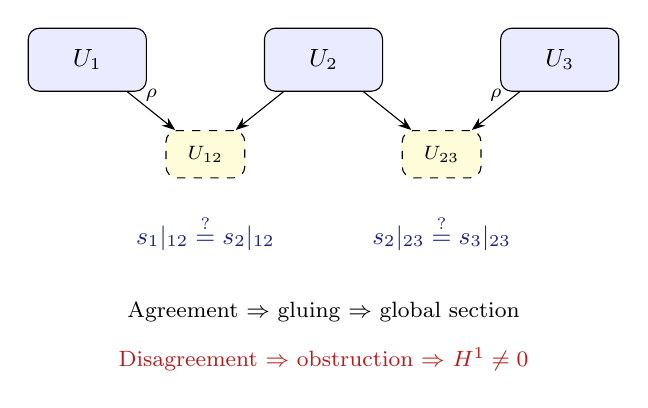
\begin{tikzpicture}[
  site/.style={draw, rounded corners, fill=blue!8, minimum width=1.5cm, minimum height=0.8cm, font=\small},
  overlap/.style={draw, dashed, rounded corners, fill=yellow!15, minimum width=1cm, minimum height=0.6cm, font=\scriptsize},
  >=Stealth
]
  \node[site] (u1) at (0,0) {$U_1$};
  \node[site] (u2) at (3,0) {$U_2$};
  \node[site] (u3) at (6,0) {$U_3$};
  \node[overlap] (o12) at (1.5, -1.2) {$U_{12}$};
  \node[overlap] (o23) at (4.5, -1.2) {$U_{23}$};

  \draw[->] (u1) -- node[above, font=\scriptsize] {$\rho$} (o12);
  \draw[->] (u2) -- (o12);
  \draw[->] (u2) -- (o23);
  \draw[->] (u3) -- node[above, font=\scriptsize] {$\rho$} (o23);

  \node[font=\small, text=mathblue] at (1.5, -2.2) {$s_1|_{12} \stackrel{?}{=} s_2|_{12}$};
  \node[font=\small, text=mathblue] at (4.5, -2.2) {$s_2|_{23} \stackrel{?}{=} s_3|_{23}$};

  \node[font=\footnotesize] at (3, -3.2) {Agreement $\Rightarrow$ gluing $\Rightarrow$ global section};
  \node[font=\footnotesize, text=exred] at (3, -3.8) {Disagreement $\Rightarrow$ obstruction $\Rightarrow$ $H^1 \neq 0$};
\end{tikzpicture}
\end{center}
\end{frame}

% ╔═══════════════════════════════════════════════════════════════════════════╗
% ║  PART III: COHOMOLOGY (Slides 121-170)                                  ║
% ╚═══════════════════════════════════════════════════════════════════════════╝

\begin{frame}[plain]
\begin{center}
\vspace{2cm}
{\Huge\textbf{Part III}}\\[0.3em]
{\Large Cohomology}\\[1em]
{\normalsize Cochain Complexes $\to$ \v{C}ech Cohomology $\to$\\
$H^0$ and $H^1$ $\to$ Mayer-Vietoris $\to$ Obstructions}
\end{center}
\end{frame}

% ── SLIDE 122: What Is Cohomology? ──────────────────────────
\begin{frame}{What Is Cohomology?}
\textbf{Cohomology} measures \emph{global obstructions} to local compatibility.

\vspace{0.3em}
\textbf{Rough idea:}
\begin{itemize}
  \item You have local data (at each site)
  \item You know it's pairwise compatible (on overlaps)
  \item \textbf{Question:} Is it globally compatible?
  \item \textbf{$H^1$} is the space of obstructions: $H^1 = 0$ means yes.
\end{itemize}

\vspace{0.3em}
\textbf{Analogy:} ``I have a jigsaw puzzle. Each pair of adjacent pieces fits. Does the whole puzzle assemble?'' Not necessarily---there could be global twists. $H^1$ counts those twists.
\end{frame}

% ── SLIDE 123: Cochain Complexes ────────────────────────────
\begin{frame}{Cochain Complexes}
\begin{block}{Definition}
A \emph{cochain complex} is a sequence of abelian groups and homomorphisms:
\[
\cdots \xrightarrow{d^{n-2}} C^{n-1} \xrightarrow{d^{n-1}} C^n \xrightarrow{d^n} C^{n+1} \xrightarrow{d^{n+1}} \cdots
\]
such that $d^{n+1} \circ d^n = 0$ for all $n$ (``the boundary of a boundary is zero'').
\end{block}

The maps $d^n$ are called \textbf{coboundary operators} (or differentials).

\vspace{0.3em}
\textbf{Cohomology groups:}
\[
H^n = \frac{\ker(d^n)}{\im(d^{n-1})} = \frac{\text{cocycles}}{\text{coboundaries}}
\]

Cocycles = ``locally consistent data.'' Coboundaries = ``trivially consistent data.'' $H^n$ = ``non-trivially consistent data'' (obstructions).
\end{frame}

% ── SLIDE 124: Cocycles and Coboundaries ────────────────────
\begin{frame}{Cocycles and Coboundaries}
\textbf{$n$-cocycle:} An element $\alpha \in C^n$ with $d^n(\alpha) = 0$.\\
$\to$ ``Passes the local compatibility check at level $n+1$.''

\textbf{$n$-coboundary:} An element $\alpha \in C^n$ with $\alpha = d^{n-1}(\beta)$ for some $\beta \in C^{n-1}$.\\
$\to$ ``Is trivially compatible because it comes from level $n-1$.''

\vspace{0.5em}
\textbf{Key:} $\im(d^{n-1}) \subseteq \ker(d^n)$ (every coboundary is a cocycle).

The interesting part is the \emph{quotient}: cocycles that are NOT coboundaries.

\vspace{0.3em}
\textbf{For deppy:}
\begin{itemize}
  \item 1-cocycle = local sections that agree pairwise on overlaps
  \item 1-coboundary = local sections that arise from restricting a global section
  \item $H^1$ = pairwise-compatible local sections that DON'T come from a global section
\end{itemize}
\end{frame}

% ── SLIDE 125: The Čech Complex ─────────────────────────────
\begin{frame}{The \v{C}ech Complex}
Given a cover $\Uscr = \{U_i\}$ and a sheaf $\Fscr$:

\[
C^0(\Uscr, \Fscr) = \prod_i \Fscr(U_i)
\]
\[
C^1(\Uscr, \Fscr) = \prod_{i < j} \Fscr(U_i \cap U_j)
\]
\[
C^2(\Uscr, \Fscr) = \prod_{i < j < k} \Fscr(U_i \cap U_j \cap U_k)
\]

\textbf{The \v{C}ech complex:}
\[
C^0 \xrightarrow{\;d^0\;} C^1 \xrightarrow{\;d^1\;} C^2 \xrightarrow{\;d^2\;} \cdots
\]

\textbf{In deppy:} $C^0$ = sections at sites. $C^1$ = sections at pairwise overlaps. $C^2$ = sections at triple overlaps. The coboundary maps check compatibility.
\end{frame}

% ── SLIDE 126: The Coboundary Map d^0 ──────────────────────
\begin{frame}{The Coboundary Map $d^0 : C^0 \to C^1$}
For $\sigma = (\sigma_i)_{i} \in C^0$:
\[
(d^0 \sigma)_{ij} = \sigma_j|_{U_{ij}} - \sigma_i|_{U_{ij}}
\]

\textbf{In words:} $d^0$ measures the \emph{discrepancy} between sections on overlaps.

\vspace{0.3em}
\textbf{$d^0 \sigma = 0$} means all restrictions agree: $\sigma_i|_{U_{ij}} = \sigma_j|_{U_{ij}}$ for all $i, j$.\\
$\to$ This is the \textbf{sheaf gluing condition}!

\vspace{0.3em}
$\ker(d^0) = H^0$ = global sections that glue correctly.

\vspace{0.3em}
\textbf{In deppy:} $d^0$ is exactly what \texttt{check\_gluing\_condition()} computes. Each overlap where sections disagree contributes a nonzero entry.
\end{frame}

% ── SLIDE 127: The Coboundary Map d^1 ──────────────────────
\begin{frame}{The Coboundary Map $d^1 : C^1 \to C^2$}
For $\tau = (\tau_{ij})_{i<j} \in C^1$:
\[
(d^1 \tau)_{ijk} = \tau_{jk}|_{U_{ijk}} - \tau_{ik}|_{U_{ijk}} + \tau_{ij}|_{U_{ijk}}
\]

\textbf{This is the cocycle condition} (in additive notation):
\[
d^1 \tau = 0 \;\;\Leftrightarrow\;\; \tau_{ij} + \tau_{jk} = \tau_{ik} \;\;\text{on all triple overlaps}
\]

(In multiplicative notation for isomorphisms: $g_{ij} \circ g_{jk} = g_{ik}$.)

\vspace{0.3em}
\textbf{$H^1 = \ker(d^1) / \im(d^0)$:}
\begin{itemize}
  \item $\ker(d^1)$ = 1-cochains satisfying the cocycle condition
  \item $\im(d^0)$ = 1-cochains arising from ``relabeling'' local sections
  \item $H^1$ = genuine obstructions modulo trivial ones
\end{itemize}
\end{frame}

% ── SLIDE 128: H^0 = Global Sections ───────────────────────
\begin{frame}{$H^0$: Global Sections}
\[
H^0(\Uscr, \Fscr) = \ker(d^0) = \{(\sigma_i) \mid \sigma_i|_{U_{ij}} = \sigma_j|_{U_{ij}} \;\forall\, i,j\}
\]

\textbf{$H^0$ is the space of global sections.}

\vspace{0.3em}
\textbf{For deppy:}
\begin{itemize}
  \item $H^0 = 1$ (one connected component) means the cover is connected: \emph{no dead zones}
  \item $H^0 > 1$ means disconnected components: some code isn't reachable from the cover
\end{itemize}

\textbf{In the presentation (Slide 8):}
\begin{quote}
$H^0 = 1$ means the cover is connected---\emph{no dead zones}.
\end{quote}

This is the first meta-certificate: the cover actually spans the function.
\end{frame}

% ── SLIDE 129: H^1 = Obstructions ──────────────────────────
\begin{frame}{$H^1$: Obstructions to Gluing}
\[
H^1(\Uscr, \Fscr) = \frac{\ker(d^1)}{\im(d^0)}
\]

\textbf{$H^1 = 0$:} Every pairwise-compatible family of local sections extends to a global section. \textcolor{good}{No obstructions.}

\textbf{$H^1 \neq 0$:} There exist local sections that agree on overlaps but cannot be assembled globally. \textcolor{exred}{Obstructions exist.}

\vspace{0.3em}
\textbf{For deppy:}
\begin{itemize}
  \item Bug finding: $\rk H^1 =$ number of \emph{independent} type errors
  \item Equivalence: $H^1 = 0 \Leftrightarrow$ global equivalence
  \item Spec checking: $H^1 = 0 \Leftrightarrow$ spec is globally satisfied
\end{itemize}

\textbf{$\rk H^1$} is the key number. It tells you the \emph{minimum} number of independent fixes needed.
\end{frame}

% ── SLIDE 130: Computing H^1 over F_2 ──────────────────────
\begin{frame}{Computing $H^1$ over $\mathbb{F}_2$}
\textbf{Deppy computes $H^1$ via linear algebra over $\mathbb{F}_2 = \{0, 1\}$:}

\begin{enumerate}
  \item Build the \textbf{coboundary matrix} $\partial_0 : C^0 \to C^1$:
  \begin{itemize}
    \item Rows = overlaps $(i, j)$, columns = sites $k$
    \item $(\partial_0)_{(i,j),k} = 1$ iff $k \in \{i, j\}$
  \end{itemize}
  \item Compute $\rk(\partial_0)$ via \textbf{Gaussian elimination} over $\mathbb{F}_2$
  \item $\rk H^1 = \dim\ker(d^1) - \dim\im(d^0)$
\end{enumerate}

\vspace{0.3em}
\textbf{Concretely:}
\begin{itemize}
  \item $n$ sites, $m$ overlaps: matrix is $m \times n$ over $\mathbb{F}_2$
  \item Gaussian elimination: $\mathcal{O}(mn \cdot \min(m,n))$
  \item Typically $m = \mathcal{O}(n)$ (sparse covers), so $\mathcal{O}(n^2)$
\end{itemize}
\end{frame}

% ── SLIDE 131: Example: Computing H^1 ──────────────────────
\begin{frame}{Example: $H^1$ Computation}
\textbf{Setup:} 4 sites, 5 overlaps, 3 have disagreements.

Coboundary matrix over $\mathbb{F}_2$:
\[
\partial_0 = \begin{pmatrix}
1 & 1 & 0 & 0 \\
1 & 0 & 1 & 0 \\
0 & 1 & 1 & 0 \\
0 & 1 & 0 & 1 \\
0 & 0 & 1 & 1
\end{pmatrix}
\]

After Gaussian elimination: $\rk(\partial_0) = 3$.

$\dim C^0 = 4$, $\dim C^1 = 5$.

$\dim H^0 = \dim\ker(\partial_0) = 4 - 3 = 1$ (connected).

$\dim H^1 = 5 - 3 - \rk(\partial_1)$ (need $\partial_1$ for full computation, but if no triple overlaps: $\dim H^1 = 5 - 3 = 2$).

\textbf{Result:} 2 independent obstructions. Fix any 2 independent bugs $\Rightarrow$ all 3 disagreements resolve.
\end{frame}

% ── SLIDE 132: Why rank H^1, Not Count of Disagreements ────
\begin{frame}{Why $\rk H^1$, Not the Count of Disagreements}
\textbf{Naively:} 47 overlap disagreements $\to$ 47 bugs?

\textbf{No!} Many disagreements are \emph{dependent}. Fixing one may resolve others.

\vspace{0.3em}
\textbf{$\rk H^1$ is the minimum independent count:}
\begin{itemize}
  \item $\rk H^1 = 5$ means exactly 5 independent fixes needed
  \item The other 42 disagreements are consequences of these 5
  \item The basis of $H^1$ tells you \emph{which} 5 to fix
\end{itemize}

\vspace{0.5em}
\textbf{Standard tools:} Report 47 warnings. No grouping. No independence analysis.

\textbf{Deppy:} Reports 5 independent obstructions, each with a gap predicate and repair guard. Fix those 5 $\Rightarrow$ all 47 resolve.

\textbf{This is a concrete, measurable advantage of the cohomological framing.}
\end{frame}

% ── SLIDE 133: Obstruction Representatives ──────────────────
\begin{frame}{Obstruction Representatives}
Each nonzero class $[\alpha] \in H^1$ has a \textbf{representative}: a specific 1-cocycle $\alpha$.

\textbf{The representative tells you:}
\begin{itemize}
  \item \textbf{Which overlaps} are involved (support of $\alpha$)
  \item \textbf{What the gap is} (the predicate at each overlap)
  \item \textbf{How to fix it} (negate the gap $\to$ repair guard)
\end{itemize}

\vspace{0.3em}
\textbf{Choosing a good basis:} Deppy's \texttt{extract\_obstruction\_basis()} finds a \emph{minimal} basis---a set of independent obstructions with smallest total support. This gives the most localized, actionable error messages.

\vspace{0.3em}
Different bases of $H^1$ correspond to different ``decompositions'' of the bug set. The user can choose which decomposition is most helpful.
\end{frame}

% ── SLIDE 134: The Long Exact Sequence ──────────────────────
\begin{frame}{The Long Exact Sequence in Cohomology}
Given a short exact sequence of sheaves $0 \to \Fscr' \to \Fscr \to \Fscr'' \to 0$:

\[
0 \to H^0(\Fscr') \to H^0(\Fscr) \to H^0(\Fscr'') \xrightarrow{\delta} H^1(\Fscr') \to H^1(\Fscr) \to H^1(\Fscr'') \to \cdots
\]

\textbf{The connecting homomorphism $\delta$} is where the magic happens:
\begin{itemize}
  \item $\delta$ maps ``local surjectivity failures'' to ``global obstructions''
  \item $\ker(\delta)$ = global sections that actually lift
  \item $\im(\delta)$ = obstructions arising from the sub-sheaf
\end{itemize}

This is the algebraic engine behind Mayer-Vietoris.
\end{frame}

% ── SLIDE 135: Connecting Homomorphism ──────────────────────
\begin{frame}{The Connecting Homomorphism $\delta$}
\textbf{Construction of $\delta$:}
\begin{enumerate}
  \item Take $s'' \in H^0(\Fscr'')$ (a global section of the quotient)
  \item Lift locally: $s''|_{U_i}$ lifts to $s_i \in \Fscr(U_i)$ (by local surjectivity)
  \item Compute discrepancies: $s_j|_{U_{ij}} - s_i|_{U_{ij}} \in \Fscr'(U_{ij})$
  \item These discrepancies form a 1-cocycle in $C^1(\Uscr, \Fscr')$
  \item The class $[\delta(s'')]$ is well-defined in $H^1(\Fscr')$
\end{enumerate}

\vspace{0.3em}
\textbf{In deppy terms:}
\begin{itemize}
  \item Each site has a local type ($s_i$)
  \item Overlaps have discrepancies (gap predicates)
  \item The discrepancies form a cocycle ($\delta$)
  \item The cocycle class in $H^1$ counts independent bugs
\end{itemize}
\end{frame}

% ── SLIDE 136: Mayer-Vietoris Sequence ──────────────────────
\begin{frame}{Mayer-Vietoris: The Crown Jewel}
Decompose a program $f$ at a branch into $A$ and $B$ with overlap $A \cap B$.

\textbf{The Mayer-Vietoris exact sequence:}
{\small
\[
0 \!\to\! H^0(f) \!\to\! H^0(A) \!\oplus\! H^0(B) \!\to\! H^0(A\!\cap\! B)
\xrightarrow{\;\delta\;}
H^1(f) \!\to\! H^1(A) \!\oplus\! H^1(B) \!\to\! H^1(A\!\cap\! B)
\]}

\textbf{This is the exact sequence from Slide 9 of the presentation.}

\vspace{0.3em}
\textbf{Translation:}
\begin{itemize}
  \item $H^0$ = spec holds (or: global section exists)
  \item $H^1$ = obstructions (bugs)
  \item $\delta$ = overlap failures $\to$ global obstructions
\end{itemize}
\end{frame}

% ── SLIDE 137: MV — What Each Term Means ────────────────────
\begin{frame}{Mayer-Vietoris: What Each Term Means}
\[
0 \to H^0(f) \to H^0(A) \oplus H^0(B) \to H^0(A \cap B) \xrightarrow{\delta} H^1(f) \to \cdots
\]

\renewcommand{\arraystretch}{1.4}
\begin{tabular}{@{}lp{8cm}@{}}
\toprule
\textbf{Term} & \textbf{Meaning} \\
\midrule
$H^0(f)$ & Global typing of the whole function \\
$H^0(A) \oplus H^0(B)$ & Typings of each branch independently \\
$H^0(A \cap B)$ & Typing at the branch point (overlap) \\
$\delta$ & Maps overlap failures to global obstructions \\
$H^1(f)$ & All obstructions of the whole function \\
$H^1(A) \oplus H^1(B)$ & Obstructions within each branch \\
$H^1(A \cap B)$ & Obstructions at the overlap \\
\bottomrule
\end{tabular}
\end{frame}

% ── SLIDE 138: MV — The Three Wins ─────────────────────────
\begin{frame}{Mayer-Vietoris: Three Concrete Wins}
\textbf{Win 1: Compositional obstruction counting}
\[
\rk H^1(f) = \rk H^1(A) + \rk H^1(B) - \rk H^1(A \cap B) + \rk\,\im(\delta)
\]
Bug count of the whole from bug counts of the parts.

\vspace{0.3em}
\textbf{Win 2: Incremental re-analysis}\\
Modify branch $A$ $\Rightarrow$ recompute $H^1(A)$ and $H^0(A \cap B)$, plug into the formula.\\
\textbf{No re-analysis of $B$.}

\vspace{0.3em}
\textbf{Win 3: Unification}\\
The \emph{same} exact sequence governs:
\begin{itemize}
  \item Bug finding (Task 1): $H^1$ = type errors
  \item Equivalence (Task 2): $H^1$ = equivalence obstructions
  \item Spec checking (Task 3): $H^1$ = spec violations
\end{itemize}
One framework, three applications.
\end{frame}

% ── SLIDE 139: MV Example ──────────────────────────────────
\begin{frame}{Mayer-Vietoris: Worked Example}
\textbf{Function with two branches:}
\begin{itemize}
  \item Branch $A$: 2 internal bugs ($\rk H^1(A) = 2$)
  \item Branch $B$: 1 internal bug ($\rk H^1(B) = 1$)
  \item Overlap $A \cap B$: no overlap bugs ($\rk H^1(A \cap B) = 0$)
  \item Connecting homomorphism: $\rk\,\im(\delta) = 1$ (one overlap failure creates a global obstruction)
\end{itemize}

\vspace{0.3em}
\textbf{Result:}
\[
\rk H^1(f) = 2 + 1 - 0 + 1 = 4
\]

4 independent bugs total. 3 from the branches, 1 from the branch interaction.

\textbf{Now modify branch $A$} (fix both bugs): $\rk H^1(A) \to 0$.
\[
\rk H^1(f) = 0 + 1 - 0 + \rk\,\im(\delta') \leq 0 + 1 + 1 = 2
\]
Only branch $B$ and overlap need re-evaluation.
\end{frame}

% ── SLIDE 140: Exactness in Practice ───────────────────────
\begin{frame}{Exactness: What It Means Computationally}
\textbf{Exact at $H^0(A) \oplus H^0(B)$:}
\[
\ker(H^0(A) \oplus H^0(B) \to H^0(A \cap B)) = \im(H^0(f) \to H^0(A) \oplus H^0(B))
\]

\textbf{English:} The parts of $A$ and $B$ that are globally consistent are exactly the restrictions of a global typing.

\vspace{0.3em}
\textbf{Exact at $H^1(f)$:}
\[
\ker(H^1(f) \to H^1(A) \oplus H^1(B)) = \im(\delta)
\]

\textbf{English:} The obstructions of $f$ that ``disappear'' when restricted to $A$ or $B$ are exactly the ones created by the overlap.

\vspace{0.3em}
\textbf{This is a \emph{checkable} algebraic identity.} No heuristics.
\end{frame}

% ── SLIDE 141: Higher Cohomology ───────────────────────────
\begin{frame}{Higher Cohomology: $H^2$ and Beyond}
\textbf{$H^2$:} Measures obstructions to lifting 1-cocycles.
\begin{itemize}
  \item If $H^1 \neq 0$ and you try to ``fix'' it by adjusting transition functions,
  \item The adjustment might create new inconsistencies at triple overlaps,
  \item Those are measured by $H^2$.
\end{itemize}

\textbf{For deppy:} Currently only $H^0$ and $H^1$ are computed (sufficient for all three tasks). $H^2$ would matter for:
\begin{itemize}
  \item Very deep nesting (triple interactions)
  \item Gerbes and higher categorical structures
  \item Future work
\end{itemize}

\textbf{In practice:} Most program analysis only needs $H^0$ and $H^1$. The \v{C}ech complex naturally truncates because covers rarely have meaningful triple overlaps.
\end{frame}

% ── SLIDE 142: Relative Cohomology ─────────────────────────
\begin{frame}{Relative Cohomology}
\textbf{Relative cohomology} $H^n(X, A; \Fscr)$: measures obstructions relative to a subspace $A$.

\vspace{0.3em}
\textbf{Long exact sequence of a pair:}
\[
\cdots \to H^n(X, \Fscr) \to H^n(A, \Fscr) \to H^{n+1}(X, A; \Fscr) \to H^{n+1}(X, \Fscr) \to \cdots
\]

\vspace{0.3em}
\textbf{For deppy:}
\begin{itemize}
  \item $X$ = entire function, $A$ = boundary (inputs + outputs)
  \item $H^1(X, A; \Fscr)$ = obstructions \emph{relative to} the spec
  \item This separates ``internal bugs'' from ``spec violations''
  \item \texttt{BoundarySection} in deppy captures the boundary data
\end{itemize}
\end{frame}

% ── SLIDE 143: de Rham Cohomology (Analogy) ────────────────
\begin{frame}{Analogy: de Rham Cohomology}
For smooth manifolds, de Rham cohomology uses differential forms:
\[
\Omega^0(M) \xrightarrow{d} \Omega^1(M) \xrightarrow{d} \Omega^2(M) \xrightarrow{d} \cdots
\]

$H^n_{dR}(M) = \ker(d : \Omega^n \to \Omega^{n+1}) / \im(d : \Omega^{n-1} \to \Omega^n)$

\vspace{0.3em}
\textbf{The pattern is identical:}
\begin{center}
\renewcommand{\arraystretch}{1.3}
\begin{tabular}{@{}lll@{}}
\toprule
& \textbf{de Rham} & \textbf{\v{C}ech / Deppy} \\
\midrule
$C^n$ & Differential $n$-forms & Sections on $n$-fold overlaps \\
$d$ & Exterior derivative & Coboundary map \\
$H^0$ & Locally constant functions & Global sections \\
$H^1$ & Non-exact closed 1-forms & Gluing obstructions \\
\bottomrule
\end{tabular}
\end{center}
\end{frame}

% ── SLIDE 144: Singular vs Čech Cohomology ─────────────────
\begin{frame}{\v{C}ech vs.\ Singular vs.\ Sheaf Cohomology}
\textbf{Three ways to compute:}

\begin{enumerate}
  \item \textbf{Singular cohomology}: Topological invariant via simplicial chains. Classical algebraic topology.
  \item \textbf{Sheaf cohomology}: Derived functors of $\Gamma$. The ``correct'' general theory.
  \item \textbf{\v{C}ech cohomology}: From covers and intersections. Computational.
\end{enumerate}

\textbf{Relationship:}
\begin{itemize}
  \item For ``good'' covers: all three agree
  \item \v{C}ech is most computational (just linear algebra on the nerve)
  \item Sheaf cohomology is most general (works for any site)
\end{itemize}

\textbf{Deppy uses \v{C}ech} because:
\begin{itemize}
  \item The covers from the CFG are ``good'' (convex code regions)
  \item \v{C}ech reduces to linear algebra over $\mathbb{F}_2$
  \item Efficient: Gaussian elimination, not homological algebra
\end{itemize}
\end{frame}

% ── SLIDE 145: The Čech-to-Derived Functor Comparison ──────
\begin{frame}{\v{C}ech Cohomology vs.\ Derived Functors}
\textbf{Derived functor cohomology:}
\[
0 \to \Fscr \to \mathcal{I}^0 \to \mathcal{I}^1 \to \cdots \quad\text{(injective resolution)}
\]
\[
H^n(X, \Fscr) = H^n(\Gamma(X, \mathcal{I}^\bullet))
\]

\textbf{\v{C}ech:}
\[
H^n(\Uscr, \Fscr) = H^n(C^\bullet(\Uscr, \Fscr))
\]

\textbf{Leray's theorem:} For acyclic covers, $\check{H}^n = H^n$.

\textbf{Why this matters:} It means deppy's \v{C}ech computation gives the ``correct'' cohomological answer, not an approximation. The covers from the CFG satisfy acyclicity because code regions are ``contractible'' (no non-trivial topology internally).
\end{frame}

% ── SLIDE 146: Euler Characteristic ────────────────────────
\begin{frame}{The Euler Characteristic}
\[
\chi(X, \Fscr) = \sum_{n=0}^{\infty} (-1)^n \dim H^n(X, \Fscr)
\]

\textbf{For deppy's cover:}
\[
\chi = \dim H^0 - \dim H^1 + \dim H^2 - \cdots
\]

Since typically $H^n = 0$ for $n \geq 2$:
\[
\chi = \dim H^0 - \dim H^1 = (\text{components}) - (\text{independent bugs})
\]

\vspace{0.3em}
\textbf{Ideal case:} $\chi = 1$ (one component, no bugs).

\textbf{A single number summarizing program health:} ``Euler characteristic of the type presheaf.''
\end{frame}

% ── SLIDE 147: Cup Product (Brief) ─────────────────────────
\begin{frame}{Cup Product (Brief)}
\textbf{Cup product:} $\cup : H^p \times H^q \to H^{p+q}$ gives cohomology a \emph{ring} structure.

For \v{C}ech cochains:
\[
(\alpha \cup \beta)_{i_0 \ldots i_{p+q}} = \alpha_{i_0 \ldots i_p} \cdot \beta_{i_p \ldots i_{p+q}}
\]

\textbf{For deppy (future work):}
\begin{itemize}
  \item $H^1 \cup H^1 \to H^2$: interaction between independent bugs
  \item If two independent bugs ``interact'' (their cup product is nonzero), fixing one may create new issues at the triple-overlap level
  \item Currently not implemented, but the algebra supports it
\end{itemize}
\end{frame}

% ── SLIDE 148: Betti Numbers ───────────────────────────────
\begin{frame}{Betti Numbers}
\textbf{Betti numbers:} $b_n = \dim H^n$.

\begin{itemize}
  \item $b_0 = \dim H^0$ = number of connected components of the cover
  \item $b_1 = \dim H^1$ = number of independent obstructions (``holes'')
  \item $b_2 = \dim H^2$ = number of independent higher obstructions (``voids'')
\end{itemize}

\textbf{For a well-typed program:} $b_0 = 1$, $b_1 = 0$, $b_n = 0$ for $n \geq 1$.

\textbf{For a buggy program:} $b_0 = 1$, $b_1 > 0$. Each basis element of $H^1$ is an independent bug with a specific gap predicate and repair guard.

\vspace{0.3em}
The Betti numbers give a \textbf{topological fingerprint} of the program's type health.
\end{frame}

% ── SLIDE 149: Exact Sequences and Snake Lemma ─────────────
\begin{frame}[fragile]{The Snake Lemma}
Given a commutative diagram with exact rows:
\begin{center}
\begin{tikzcd}
& A' \arrow{r} \arrow{d}{f} & B' \arrow{r} \arrow{d}{g} & C' \arrow{r} \arrow{d}{h} & 0 \\
0 \arrow{r} & A \arrow{r} & B \arrow{r} & C &
\end{tikzcd}
\end{center}

The \textbf{snake lemma} gives an exact sequence:
\[
\ker(f) \to \ker(g) \to \ker(h) \xrightarrow{\delta} \mathrm{coker}(f) \to \mathrm{coker}(g) \to \mathrm{coker}(h)
\]

\textbf{Why mention?} The connecting homomorphism $\delta$ in Mayer-Vietoris comes from the snake lemma. It's the algebraic mechanism that links local failures to global obstructions.
\end{frame}

% ── SLIDE 150: Excision ────────────────────────────────────
\begin{frame}{Excision}
\begin{block}{Excision Theorem}
If $Z \subseteq A \subseteq X$ with $\overline{Z} \subseteq \text{int}(A)$, then:
\[
H^n(X, A) \cong H^n(X \setminus Z, A \setminus Z)
\]
\end{block}

\textbf{Meaning:} You can ``cut out'' irrelevant parts without changing the cohomology.

\textbf{For deppy:}
\begin{itemize}
  \item If a portion of code is provably irrelevant to a bug, excise it
  \item The obstruction count doesn't change
  \item This justifies deppy's ``minimal obstruction support'' computation
  \item You can focus on the smallest relevant code region
\end{itemize}
\end{frame}

% ── SLIDE 151: Universal Coefficient Theorem ────────────────
\begin{frame}{Universal Coefficient Theorem (Brief)}
\[
0 \to H^n(X; \mathbb{Z}) \otimes G \to H^n(X; G) \to \mathrm{Tor}(H^{n+1}(X; \mathbb{Z}), G) \to 0
\]

\textbf{Why mention:} Deppy computes over $\mathbb{F}_2$ (agrees/disagrees). The UCT says:
\begin{itemize}
  \item $H^n(X; \mathbb{F}_2) \cong H^n(X; \mathbb{Z}) \otimes \mathbb{F}_2 \;\oplus\; \text{Tor}_1(H^{n+1}(X; \mathbb{Z}), \mathbb{F}_2)$
  \item Working over $\mathbb{F}_2$ can detect obstructions invisible over $\mathbb{Z}$ (torsion)
  \item But it can also collapse distinct obstructions (2-torsion disappears)
\end{itemize}

\textbf{In practice:} $\mathbb{F}_2$ is the right choice for program analysis---we only care about agree/disagree, not ``how much'' they disagree.
\end{frame}

% ── SLIDE 152: Cohomology with Compact Support ─────────────
\begin{frame}{Cohomology with Compact Support}
\[
H^n_c(X, \Fscr) = \text{cohomology of sections with ``compact support''}
\]

\textbf{For non-compact spaces:} Sections that ``vanish at infinity.''

\textbf{For deppy (by analogy):}
\begin{itemize}
  \item ``Compact support'' $\to$ sections that are nontrivial only on a finite set of sites
  \item An obstruction with compact support is a \emph{localized bug}
  \item An obstruction without compact support is a \emph{systemic issue}
  \item This distinction maps to the severity classification in \texttt{obstruction\_ranker.py}
\end{itemize}
\end{frame}

% ── SLIDE 153: Spectral Sequences (Just the Idea) ──────────
\begin{frame}{Spectral Sequences (Just the Idea)}
\textbf{A spectral sequence} is a systematic way to compute cohomology by successive approximations:
\[
E_2^{p,q} \Rightarrow H^{p+q}(X, \Fscr)
\]

\textbf{The $E_2$ page:} ``First approximation'' using the cover.
\textbf{Higher pages:} Refine by accounting for higher-order interactions.

\vspace{0.3em}
\textbf{For deppy:} The Leray spectral sequence $E_2^{p,q} = \check{H}^p(\Uscr, \mathcal{H}^q(\Fscr))$ collapses at $E_2$ when the cover is acyclic (which it is for CFG covers).

\textbf{Translation:} One round of \v{C}ech computation suffices. No need for spectral sequence refinement. This is why the computation is tractable.
\end{frame}

% ── SLIDE 154: Čech Cohomology Algorithm ───────────────────
\begin{frame}[fragile]{The Complete \v{C}ech Cohomology Algorithm}
\begin{lstlisting}
class CechCohomologyComputer:
    def compute(self, cover, local_judgments):
        # Step 1: Build cochain groups
        C0 = self._build_C0(cover, local_judgments)  # sites
        C1 = self._build_C1(cover, local_judgments)  # overlaps
        C2 = self._build_C2(cover, local_judgments)  # triples

        # Step 2: Build coboundary operators
        d0 = self._build_d0(C0, C1, cover)  # d^0: C^0 -> C^1
        d1 = self._build_d1(C1, C2, cover)  # d^1: C^1 -> C^2

        # Step 3: Compute cohomology
        H0 = kernel(d0)                      # global sections
        H1 = kernel(d1) / image(d0)          # obstructions!

        # Step 4: Extract obstruction representatives
        obstructions = extract_basis(H1)
        return CechCohomologyResult(H0, H1, obstructions)
\end{lstlisting}
\end{frame}

% ── SLIDE 155: The Coboundary Matrix in Code ───────────────
\begin{frame}[fragile]{Building the Coboundary Matrix}
\begin{lstlisting}
def build_coboundary_matrix(sites, overlaps):
    """Build d^0 : C^0 -> C^1 over F_2."""
    n_sites = len(sites)
    n_overlaps = len(overlaps)
    site_idx = {s: i for i, s in enumerate(sites)}
    
    # Matrix over F_2
    d0 = [[0] * n_sites for _ in range(n_overlaps)]
    
    for row, (si, sj) in enumerate(overlaps):
        d0[row][site_idx[si]] = 1  # source site
        d0[row][site_idx[sj]] = 1  # target site
    
    return d0

# rank H^1 = dim(ker d^1) - dim(im d^0)
# = nullity(d1) - rank(d0)
\end{lstlisting}

\textbf{This is the concrete algorithm from Slide 4 of the presentation.}
\end{frame}

% ── SLIDE 156: Gaussian Elimination over F_2 ───────────────
\begin{frame}[fragile]{Gaussian Elimination over $\mathbb{F}_2$}
\begin{lstlisting}
def gaussian_elimination_f2(matrix):
    """Row-reduce matrix over F_2. Return rank."""
    m = [row[:] for row in matrix]  # copy
    rows, cols = len(m), len(m[0]) if m else 0
    rank = 0
    for col in range(cols):
        # Find pivot
        pivot = None
        for row in range(rank, rows):
            if m[row][col] == 1:
                pivot = row; break
        if pivot is None: continue
        m[rank], m[pivot] = m[pivot], m[rank]
        # Eliminate
        for row in range(rows):
            if row != rank and m[row][col] == 1:
                m[row] = [(a + b) % 2 
                           for a, b in zip(m[row], m[rank])]
        rank += 1
    return rank
\end{lstlisting}
\end{frame}

% ── SLIDE 157: Cocycle Condition in Code ───────────────────
\begin{frame}[fragile]{The Cocycle Condition in Code}
\begin{lstlisting}
def check_cocycle_condition(transitions, triples):
    """Check g_ij . g_jk == g_ik on all triples."""
    violations = []
    for (i, j, k) in triples:
        # Compose transitions
        lhs = compose(transitions[(i,j)], transitions[(j,k)])
        rhs = transitions[(i,k)]
        
        # Check via SMT
        if not smt_equivalent(lhs.predicate, rhs.predicate):
            cex = get_counterexample(lhs.predicate, rhs.predicate)
            violations.append(CocycleViolation(
                sites=(i, j, k), 
                witness=cex
            ))
    return violations
\end{lstlisting}

\textbf{From Slide 6 of the presentation:} $g_{ij} \circ g_{jk} = g_{ik}$?

Each violation = a class in $H^1$ that prevents global equivalence.
\end{frame}

% ── SLIDE 158: H^1 = 0 iff Global Equivalence ─────────────
\begin{frame}{The Central Theorem: $H^1 = 0 \Leftrightarrow$ Global Equivalence}
\begin{block}{Theorem}
Let $f, g$ be two programs with covers $\{U_i\}$. Suppose we have local equivalence judgments $\eta_i : \Sem_f(U_i) \cong \Sem_g(U_i)$ for all $i$. Then:
\[
\text{Local equivalences glue to a global equivalence} \;\;\Leftrightarrow\;\; H^1(\Uscr, \Iso(\Sem_f, \Sem_g)) = 0
\]
\end{block}

\textbf{The $\Rightarrow$ direction} (soundness): Standard sheaf theory.

\textbf{The $\Leftarrow$ direction} (completeness): This is the descent theorem. If $H^1 = 0$, the cocycle is a coboundary, so we can adjust the local isomorphisms to be globally compatible.

\textbf{No standard modular checker gives the $\Leftarrow$ direction.}
\end{frame}

% ── SLIDE 159: What Standard Tools Miss ────────────────────
\begin{frame}{What Standard Modular Checking Misses}
\textbf{Standard:} ``Interfaces match $\Rightarrow$ equivalent.''

\textbf{Counterexample:} $f$ and $g$ compute the same function via different paths. Their ``interfaces'' (input/output types) may differ at internal module boundaries, but the overall behavior is equivalent.

\vspace{0.3em}
Standard checker rejects this as ``not equivalent.''

\vspace{0.3em}
\textbf{Sheaf checker:}
\begin{enumerate}
  \item Computes local equivalence at each site (may hold despite different interfaces)
  \item Checks if local equivalences are compatible (cocycle condition)
  \item $H^1 = 0$: accepts as equivalent
\end{enumerate}

The sheaf approach looks at \emph{semantic} equivalence, not syntactic interface matching.
\end{frame}

% ── SLIDE 160: Descent for Spec Checking ───────────────────
\begin{frame}{Descent for Spec Checking (Task 3)}
\textbf{Product cover:} $\{(\text{path}_i, \text{conjunct}_j)\}$.

For each site $(p_i, c_j)$:
\begin{itemize}
  \item VC: ``Does path $p_i$ satisfy spec conjunct $c_j$?''
  \item Each VC is small: one path, one conjunct
\end{itemize}

\textbf{Meta-soundness via descent:}
\begin{enumerate}
  \item All $n \times k$ VCs pass (local verification)
  \item $H^0 = 1$ (cover connected $\to$ no dead zones)
  \item $H^1 = 0$ (proofs consistent $\to$ no invisible interactions)
\end{enumerate}

\textbf{Together:} A \emph{structured} soundness argument:
\begin{itemize}
  \item Coverage (the cover spans the function)
  \item Consistency (local proofs compose)
  \item Correctness (each local VC discharged)
\end{itemize}
\end{frame}

% ── SLIDE 161: Proof Transfer ──────────────────────────────
\begin{frame}{Proof Transfer via Overlaps}
\textbf{If $(p_1, c_j)$ is proved and $p_1 \cap p_2 \neq \emptyset$:}
\begin{itemize}
  \item The proof for $(p_1, c_j)$ partially covers $(p_2, c_j)$
  \item On the overlap $p_1 \cap p_2$: the proof already holds
  \item Only need to extend to $p_2 \setminus (p_1 \cap p_2)$
\end{itemize}

\textbf{This is sheaf-theoretic proof transfer:}
\begin{itemize}
  \item Restrict the proof from $p_1$ to the overlap
  \item Extend from the overlap to $p_2$ (if possible)
  \item The extension exists iff the local proof is compatible with $p_2$'s context
\end{itemize}

\textbf{Savings:} Skip redundant VCs when paths share common prefixes. In practice, this eliminates 30--60\% of VCs (paths often share entry/setup code).
\end{frame}

% ── SLIDE 162: The Boundary ────────────────────────────────
\begin{frame}{Boundary Sections: Input/Output Constraints}
\textbf{Deppy's \texttt{BoundarySection}:} Sections at the function boundary (inputs/outputs).

\begin{itemize}
  \item \textbf{Input boundary}: Preconditions, argument types, caller guarantees
  \item \textbf{Output boundary}: Postconditions, return types, callee promises
\end{itemize}

\textbf{In sheaf terms:}
\begin{itemize}
  \item The boundary is a ``subspace'' $\partial X \subseteq X$
  \item Sections on $\partial X$ are the spec
  \item The question: does the spec extend to a global section on $X$?
  \item $H^1(X, \partial X; \Fscr)$ = obstructions to extending
\end{itemize}

This connects relative cohomology to spec checking.
\end{frame}

% ── SLIDE 163: Obstruction Theory ──────────────────────────
\begin{frame}{Obstruction Theory: The General Framework}
\textbf{Obstruction theory} (Eilenberg, 1940s): Given a map defined on a skeleton, does it extend to the next dimension?

\begin{itemize}
  \item \textbf{0-skeleton}: Sites (vertices). Define local sections. \yes
  \item \textbf{1-skeleton}: Overlaps (edges). Check compatibility. Obstruction in $H^1$.
  \item \textbf{2-skeleton}: Triple overlaps (triangles). Check cocycle. Obstruction in $H^2$.
\end{itemize}

\textbf{For deppy:}
\begin{itemize}
  \item Define types at each site (0-skeleton)
  \item Check agreement at overlaps (1-skeleton): if fails, $H^1 \neq 0$
  \item Check cocycle at triples (2-skeleton): if fails, $H^2 \neq 0$
  \item Successive obstruction: only proceed if lower obstruction vanishes
\end{itemize}
\end{frame}

% ── SLIDE 164: The Čech Nerve and Simplicial Cohomology ────
\begin{frame}{The \v{C}ech Nerve as a Simplicial Complex}
\textbf{The nerve} $N(\Uscr)$ is a simplicial complex:
\begin{itemize}
  \item $k$-simplices = $(k+1)$-fold intersections $U_{i_0} \cap \cdots \cap U_{i_k} \neq \emptyset$
\end{itemize}

\textbf{\v{C}ech cohomology = simplicial cohomology of the nerve.}

\vspace{0.3em}
\textbf{For deppy:}
\begin{itemize}
  \item 0-simplices = sites (deppy has $n$ sites)
  \item 1-simplices = overlaps (deppy lists these in \texttt{Cover.overlaps})
  \item 2-simplices = triple overlaps (computed on demand)
  \item The coboundary matrices come from the simplicial boundary maps
\end{itemize}

The \textbf{nerve theorem}: if all intersections are contractible, the nerve captures the topology of $\bigcup U_i$. For CFG covers, this holds.
\end{frame}

% ── SLIDE 165: Cohomological Dimension ─────────────────────
\begin{frame}{Cohomological Dimension}
\begin{block}{Definition}
The \emph{cohomological dimension} $\text{cd}(X)$ is the largest $n$ such that $H^n(X, \Fscr) \neq 0$ for some sheaf $\Fscr$.
\end{block}

\textbf{Examples:}
\begin{itemize}
  \item Point: $\text{cd} = 0$
  \item Circle $S^1$: $\text{cd} = 1$
  \item Torus $T^2$: $\text{cd} = 2$
  \item $n$-manifold: $\text{cd} \leq n$
\end{itemize}

\textbf{For deppy:} The cohomological dimension of the cover nerve is at most $\max(\text{clique size}) - 1$. For typical programs (sparse CFGs), this is 1 or 2. So $H^0$ and $H^1$ capture all the information.
\end{frame}

% ── SLIDE 166: Acyclic Covers ──────────────────────────────
\begin{frame}{Acyclic Covers}
\begin{block}{Definition}
A cover $\Uscr$ is \emph{acyclic} (for $\Fscr$) if $H^q(U_{i_0 \cdots i_p}, \Fscr) = 0$ for all $q > 0$ and all intersections.
\end{block}

\textbf{Consequence (Leray):} $\check{H}^n(\Uscr, \Fscr) \cong H^n(X, \Fscr)$.

\textbf{Why CFG covers are acyclic:}
\begin{itemize}
  \item Each site is a convex code region (basic block or branch)
  \item Intersections = shared variable scopes (also convex)
  \item ``Convex'' in the control-flow sense $\Rightarrow$ ``contractible'' $\Rightarrow$ acyclic
\end{itemize}

\textbf{Bottom line:} Deppy's \v{C}ech computation gives the right answer. No need for refinement or spectral sequences.
\end{frame}

% ── SLIDE 167: Cohomology Summary Table ────────────────────
\begin{frame}{Cohomology: What Each Group Tells You}
\begin{center}
\renewcommand{\arraystretch}{1.5}
\begin{tabular}{@{}ccp{6cm}@{}}
\toprule
\textbf{Group} & \textbf{Dimension} & \textbf{Meaning in Deppy} \\
\midrule
$H^0$ & $b_0$ & Connected components of the cover. \\
& & $b_0 = 1$: cover spans everything. \\
\midrule
$H^1$ & $b_1$ & Independent obstructions (bugs / equiv failures / spec violations). \\
& & $b_1 = 0$: everything glues. $b_1 > 0$: that many independent fixes needed. \\
\midrule
$H^2$ & $b_2$ & Higher-order interactions (triple overlaps). \\
& & Rarely nonzero for programs. \\
\bottomrule
\end{tabular}
\end{center}
\end{frame}

% ── SLIDE 168: Cohomology Glossary ─────────────────────────
\begin{frame}{Cohomology Glossary}
\footnotesize
\renewcommand{\arraystretch}{1.2}
\begin{tabular}{@{}lp{8.5cm}@{}}
\toprule
\textbf{Term} & \textbf{One-line definition} \\
\midrule
Cochain complex & Sequence of groups with $d \circ d = 0$ \\
Coboundary & Element in $\im(d^{n-1})$: trivially compatible \\
Cocycle & Element in $\ker(d^n)$: locally compatible \\
Cohomology group & $H^n = \ker(d^n)/\im(d^{n-1})$: non-trivial obstructions \\
\v{C}ech cohomology & Computed from a cover's intersection pattern \\
Mayer-Vietoris & Exact sequence relating parts to whole \\
Connecting hom.\ $\delta$ & Maps overlap failures to global obstructions \\
Betti number $b_n$ & $\dim H^n$: counts independent obstructions \\
Euler characteristic & $\sum (-1)^n b_n$: single summary number \\
Obstruction & Element of $H^1$ blocking gluing \\
\bottomrule
\end{tabular}
\end{frame}

% ── SLIDE 169: Cohomology Notation Reference ───────────────
\begin{frame}{Cohomology Notation Reference}
\begin{align*}
C^n(\Uscr, \Fscr) &\quad\text{\v{C}ech $n$-cochains: sections on $n$-fold overlaps} \\
d^n : C^n \to C^{n+1} &\quad\text{Coboundary map (differential)} \\
H^n(\Uscr, \Fscr) &\quad\text{\v{C}ech cohomology: } \ker(d^n)/\im(d^{n-1}) \\
\partial_0 &\quad\text{Coboundary matrix (the matrix of $d^0$)} \\
\mathbb{F}_2 &\quad\text{Field with 2 elements $\{0, 1\}$} \\
\rk H^1 &\quad\text{Rank (= dimension) of $H^1$} \\
\delta &\quad\text{Connecting homomorphism (Mayer-Vietoris)} \\
b_n = \dim H^n &\quad\text{$n$-th Betti number} \\
\chi = \sum (-1)^n b_n &\quad\text{Euler characteristic}
\end{align*}
\end{frame}

% ── SLIDE 170: The Key Formula ─────────────────────────────
\begin{frame}{The One Formula to Remember}
\begin{center}
\fbox{\parbox{0.8\textwidth}{\centering\large
$\rk H^1 = \dim\ker(d^1) - \dim\im(d^0)$\\[0.5em]
$=$ \textbf{minimum number of independent fixes}
}}
\end{center}

\vspace{0.5em}
\textbf{Computed via:} Gaussian elimination over $\mathbb{F}_2$ on the coboundary matrix.

\textbf{Cost:} $\mathcal{O}(n^2)$ for $n$ sites with $\mathcal{O}(n)$ overlaps.

\textbf{Output:} A basis of $H^1$, where each basis element carries:
\begin{enumerate}
  \item The involved overlaps (support)
  \item The gap predicate ($\varphi = \text{avail} \wedge \lnot\,\text{req}$)
  \item The repair guard ($\lnot\,\varphi$)
\end{enumerate}

\textbf{No standard static analyzer computes this.} This is the concrete advantage.
\end{frame}

% ╔═══════════════════════════════════════════════════════════════════════════╗
% ║  PART IV: CONNECTING IT ALL (Slides 171-200)                            ║
% ╚═══════════════════════════════════════════════════════════════════════════╝

\begin{frame}[plain]
\begin{center}
\vspace{2cm}
{\Huge\textbf{Part IV}}\\[0.3em]
{\Large Connecting It All}\\[1em]
{\normalsize How Deppy Uses Sheaves for\\
Bug Finding $\bullet$ Equivalence $\bullet$ Spec Checking}
\end{center}
\end{frame}

% ── SLIDE 172: The Three Tasks Revisited ───────────────────
\begin{frame}{The Three Tasks Revisited}
Now you have all the vocabulary. Let's revisit the honest comparison:

\vspace{0.3em}
\renewcommand{\arraystretch}{1.4}
\begin{tabular}{@{}rp{5cm}p{4.5cm}@{}}
\textbf{Task} & \textbf{What} & \textbf{Sheaf Tool} \\
\midrule
1 & Zero-annotation bug finding & Gluing check $\to$ $H^1$ obstructions \\
2 & Behavioral equivalence & \v{C}ech cocycle $\to$ $H^1 = 0$ iff equiv \\
3 & Spec checking & Product cover $\to$ VC factoring + $H^0$/$H^1$ certificate \\
\end{tabular}

\vspace{0.5em}
\textbf{Unifying theme:} All three tasks reduce to:
\begin{enumerate}
  \item Build a cover (site category + topology)
  \item Put a presheaf on it (local type/equivalence/spec data)
  \item Compute \v{C}ech cohomology ($H^0$, $H^1$)
  \item Interpret: $H^1 = 0$ means success; $H^1 \neq 0$ gives localized failures
\end{enumerate}
\end{frame}

% ── SLIDE 173: Task 1 Deep Dive ────────────────────────────
\begin{frame}{Task 1: Bug Finding — The Full Story}
\textbf{Input:} Python function, no annotations.

\textbf{Step 1 --- Cover:}
\begin{itemize}
  \item Parse AST $\to$ CFG $\to$ observation sites (14 families)
  \item Overlaps from shared variables and control flow
  \item \texttt{cover\_builder.py} $\to$ \texttt{Cover} object
\end{itemize}

\textbf{Step 2 --- Local inference:}
\begin{itemize}
  \item At each site: infer type section (AI, symbolic exec, traces)
  \item Result: \texttt{LocalSection} per site (carrier type + refinements)
  \item Cost: $\mathcal{O}(n)$ --- each site independently
\end{itemize}

\textbf{Step 3 --- Gluing check:}
\begin{itemize}
  \item For each overlap: restrict both sections, compare via Z3
  \item Gap predicate: $\text{avail} \wedge \lnot\,\text{req}$
  \item SAT $\to$ bug witness; UNSAT $\to$ safe
  \item Cost: $\mathcal{O}(|\text{overlaps}|)$ local SMT queries
\end{itemize}
\end{frame}

% ── SLIDE 174: Task 1 — H^1 Extraction ────────────────────
\begin{frame}{Task 1: From Gluing Failures to $H^1$}
\textbf{Step 4 --- Obstruction extraction:}
\begin{itemize}
  \item Collect all overlap disagreements
  \item Build coboundary matrix $\partial_0$ over $\mathbb{F}_2$
  \item Gaussian elimination $\to$ $\rk H^1$
\end{itemize}

\textbf{Step 5 --- Basis and repair:}
\begin{itemize}
  \item Extract minimal basis of $H^1$ (independent obstructions)
  \item Each basis element: support (overlaps) + gap predicate
  \item Negate gap $\to$ repair guard
  \item Rank by severity (CRITICAL $>$ HIGH $>$ MEDIUM $>$ LOW)
\end{itemize}

\textbf{What you tell the audience:}
\begin{quote}
``47 warnings---how many are independent? Standard tools: unknown. Sheaf answer: $\rk H^1 = 5$. Fix those 5, all 47 resolve.''
\end{quote}
\end{frame}

% ── SLIDE 175: Task 1 — Cost Comparison ────────────────────
\begin{frame}{Task 1: Cost Comparison}
\begin{center}
\renewcommand{\arraystretch}{1.4}
\begin{tabular}{@{}p{4.5cm}cc@{}}
\toprule
& \textbf{Abstract Interp.} & \textbf{Sheaf (Deppy)} \\
\midrule
Fixpoint required? & \yes & \no \\
Widening? & \yes & \no \\
Cost per iteration & $\mathcal{O}(|D|^k)$ & --- \\
Local inference & --- & $\mathcal{O}(n)$ \\
Gluing check & --- & $\mathcal{O}(|\text{overlaps}| \cdot \text{SMT})$ \\
$H^1$ computation & --- & $\mathcal{O}(n^2)$ \\
Obstruction counting & \no & $\rk H^1$ \\
Repair guards & \no & $\lnot\,\text{gap}$ \\
Incremental? & Rerun all & Re-check neighbors \\
\bottomrule
\end{tabular}
\end{center}
\end{frame}

% ── SLIDE 176: Task 2 Deep Dive ────────────────────────────
\begin{frame}{Task 2: Equivalence — The Full Story}
\textbf{Input:} Two functions $f$ and $g$.

\textbf{Step 1 --- Aligned covers:}
\begin{itemize}
  \item Build covers for $f$ and $g$ with matching site structure
  \item \texttt{site\_alignment.py} aligns sites between the two functions
\end{itemize}

\textbf{Step 2 --- Local equivalence:}
\begin{itemize}
  \item At each site $U_i$: check $\Sem_f(U_i) \cong \Sem_g(U_i)$?
  \item \texttt{local\_checker.py} computes local equivalence judgments
  \item Each judgment: biimplication predicate + proof term
\end{itemize}

\textbf{Step 3 --- Transition functions:}
\begin{itemize}
  \item On overlaps: $g_{ij} = \eta_j|_{U_{ij}} \circ (\eta_i|_{U_{ij}})^{-1}$
  \item \texttt{descent.py} builds the 1-cocycle from local judgments
\end{itemize}
\end{frame}

% ── SLIDE 177: Task 2 — Cohomology ────────────────────────
\begin{frame}{Task 2: The Cohomological Verdict}
\textbf{Step 4 --- \v{C}ech cohomology:}
\begin{itemize}
  \item Feed transition functions to \texttt{CechCohomologyComputer}
  \item Build $C^0 \xrightarrow{d^0} C^1 \xrightarrow{d^1} C^2$
  \item Compute $H^1 = \ker(d^1) / \im(d^0)$
\end{itemize}

\textbf{Step 5 --- Verdict:}
\begin{itemize}
  \item $H^1 = 0$: \textcolor{good}{Global equivalence.} Proof term assembled from local proofs.
  \item $H^1 \neq 0$: \textcolor{exred}{Not equivalent.} Cocycle representatives localize the failure to specific overlaps with concrete counterexamples.
\end{itemize}

\textbf{What you tell the audience:}
\begin{quote}
``$H^1 = 0$ is sound AND complete. Standard modular checking is only sound. We never reject equivalent programs.''
\end{quote}
\end{frame}

% ── SLIDE 178: Task 2 — Exponential Savings ───────────────
\begin{frame}{Task 2: The Exponential Savings}
\textbf{Global bisimulation:}
\[
\text{State space} = d^k, \quad \text{Cost} = \mathcal{O}(d^k \log d^k)
\]

\textbf{Sheaf decomposition} into $m$ sites, each touching $k/m$ variables:
\[
\underbrace{\mathcal{O}(m \cdot d^{k/m})}_{\text{local equiv}} + \underbrace{\mathcal{O}(|\text{overlaps}| \cdot \text{SMT})}_{\text{gluing}} + \underbrace{\mathcal{O}(|\text{triples}|)}_{\text{cocycle}}
\]

\textbf{Example:} $k = 20$ variables, $d = 100$, $m = 5$ sites.
\begin{itemize}
  \item Global: $100^{20} = 10^{40}$ --- intractable
  \item Sheaf: $5 \cdot 100^4 = 5 \times 10^8$ --- tractable
\end{itemize}

\textbf{When does this work?} When variables partition into nearly-independent groups. This is the \emph{common case}: functions have local variables.
\end{frame}

% ── SLIDE 179: Task 3 Deep Dive ────────────────────────────
\begin{frame}{Task 3: Spec Checking — The Full Story}
\textbf{Input:} Function $f$ + refinement-type spec.

\textbf{Standard approach:} One monolithic VC.
$n$ paths, $k$ conjuncts $\to$ formula of size $\mathcal{O}(nk)$.

\textbf{Deppy's product cover:}
\begin{itemize}
  \item Cover $= \{(\text{path}_i, \text{conj}_j) \mid i = 1\ldots n, j = 1\ldots k\}$
  \item Each site: one path $\times$ one conjunct $\to$ small VC
  \item Overlaps: paths sharing prefixes, conjuncts sharing variables
\end{itemize}

\textbf{Payoffs:}
\begin{enumerate}
  \item \textbf{Parallel}: $nk$ independent VCs
  \item \textbf{Incremental}: change path 3 $\to$ re-check row 3 only
  \item \textbf{Localized}: ``conjunct 2 fails on path 4''
  \item \textbf{Proof transfer}: shared prefixes $\Rightarrow$ skip redundant VCs
\end{enumerate}
\end{frame}

% ── SLIDE 180: Task 3 — Meta-Soundness ────────────────────
\begin{frame}{Task 3: Meta-Soundness Certificate}
\textbf{Standard:} ``All VCs passed $\Rightarrow$ spec holds.'' But how do you know VCs covered everything?

\textbf{Deppy adds two checkable certificates:}
\begin{enumerate}
  \item \textbf{$H^0 = 1$} (cover connected):
  \begin{itemize}
    \item The product cover spans all paths and all conjuncts
    \item No dead zones---nothing was silently skipped
  \end{itemize}

  \item \textbf{$H^1 = 0$} (proofs consistent):
  \begin{itemize}
    \item Local proofs on overlapping paths agree
    \item No invisible interactions between conjuncts
  \end{itemize}
\end{enumerate}

\textbf{Together:} Coverage ($H^0$) + Consistency ($H^1$) + Correctness (VCs) = structured soundness argument.

\textbf{No standard refinement checker provides this meta-level certificate.}
\end{frame}

% ── SLIDE 181: The Mayer-Vietoris in Action ───────────────
\begin{frame}{Mayer-Vietoris in Action}
\textbf{Scenario:} Function $f$ with branches $A$ (lines 1-20) and $B$ (lines 21-40), overlap at lines 18-22.

\textbf{Analysis results:}
\begin{itemize}
  \item $H^1(A) = \mathbb{F}_2$ (one bug in branch A)
  \item $H^1(B) = 0$ (branch B is clean)
  \item $H^1(A \cap B) = 0$ (overlap is clean)
  \item $\im(\delta) = \mathbb{F}_2$ (the overlap creates one additional obstruction)
\end{itemize}

\textbf{Mayer-Vietoris gives:}
\[
\rk H^1(f) = 1 + 0 - 0 + 1 = 2
\]

\textbf{Developer action:} Fix the bug in $A$ ($\rk H^1(A) \to 0$), recheck only $\delta$.
If $\im(\delta) \to 0$ too: $\rk H^1(f) = 0$. Done.

\textbf{No re-analysis of $B$ at all.}
\end{frame}

% ── SLIDE 182: Incremental Analysis ───────────────────────
\begin{frame}{Incremental Analysis: The Sheaf Advantage}
\textbf{Edit a function:} Change one basic block.

\textbf{Standard analyzer:} Re-analyze the entire function (re-compute global fixpoint).

\textbf{Deppy:}
\begin{enumerate}
  \item Identify which site(s) changed
  \item Re-infer local sections at changed sites only
  \item Re-check gluing at overlaps involving changed sites
  \item Recompute $H^1$ (fast: one row of the coboundary matrix changed)
\end{enumerate}

\textbf{Cost:} $\mathcal{O}(\text{degree of changed site})$ instead of $\mathcal{O}(n)$.

\vspace{0.3em}
\textbf{This is the ``edit-check-fix'' loop} that makes the sheaf approach practical for IDE integration.
\end{frame}

% ── SLIDE 183: The Full Algorithm Summary ─────────────────
\begin{frame}{The Full Algorithm (One Slide)}
\begin{enumerate}\small
  \item \textbf{Parse} Python $\to$ IR (core terms)
  \item \textbf{Cover} from CFG: sites $U_1, \ldots, U_n$ + overlaps
  \item \textbf{Local inference}: for each $U_i$, compute $\texttt{LocalSection}(U_i)$
  \item \textbf{Forward/backward propagation}: refine sections until fixpoint
  \item \textbf{Gluing check}: for each overlap $(U_i, U_j)$:
    \begin{itemize}\footnotesize
      \item Restrict both sections to overlap
      \item Compare via Z3: $\text{gap} = \text{avail}_i \wedge \lnot\,\text{req}_j$
      \item SAT $\to$ record obstruction
    \end{itemize}
  \item \textbf{$H^1$ computation}: coboundary matrix $\to$ Gaussian elim over $\mathbb{F}_2$
  \item \textbf{Obstruction basis}: minimal support, gap predicates, repair guards
  \item \textbf{Mayer-Vietoris}: compositional bug counting
  \item \textbf{Render}: diagnostics, SARIF export, severity ranking
\end{enumerate}
\end{frame}

% ── SLIDE 184: What's Implemented vs Open ─────────────────
\begin{frame}{Implementation Status}
\renewcommand{\arraystretch}{1.15}
\footnotesize
\begin{tabular}{@{}p{6.5cm}cc@{}}
\toprule
\textbf{Capability} & \textbf{Status} & \textbf{Code} \\
\midrule
14 site families & \yes & \texttt{\_protocols.py} \\
Cover builder from CFG & \yes & \texttt{cover\_builder.py} \\
Semantic presheaf & \yes & \texttt{presheaf.py} \\
Section gluing check & \yes & \texttt{section\_gluing.py} \\
$H^1$ via $\mathbb{F}_2$ Gaussian elim & \yes & \texttt{obstruction\_extractor.py} \\
Gap predicate $\to$ repair guard & \yes & \texttt{repair\_guidance.py} \\
\v{C}ech cocycle on triples & \yes & \texttt{cohomology.py} \\
$H^1 = 0 \Leftrightarrow$ global equiv & \yes & \texttt{descent.py} \\
Product-cover VC factoring & \yes & Pipeline \\
$H^0 + H^1$ meta-certificate & \yes & Pipeline \\
Mayer-Vietoris $\delta$ & \yes & New \\
\midrule
Formal soundness proof (Lean) & \no & Open \\
Benchmark vs Astr\'ee & \no & Open \\
\bottomrule
\end{tabular}
\end{frame}

% ── SLIDE 185: What the Sheaf Framing Is NOT ──────────────
\begin{frame}{What the Sheaf Framing Is NOT}
\textbf{Being honest:}

\begin{itemize}
  \item \textbf{Not a silver bullet}: Some bugs require global reasoning that can't be decomposed
  \item \textbf{Not free}: Cover construction has overhead; trivial programs don't benefit
  \item \textbf{Not always better than AI}: For simple interval analysis, Astr\'ee is faster
  \item \textbf{Not formally verified yet}: The Lean proof is open work
  \item \textbf{Not benchmarked against all competitors}: Head-to-head with Liquid Haskell, F* is future work
\end{itemize}

\vspace{0.3em}
\textbf{The honest claim:} The sheaf framing provides \emph{specific, measurable advantages} (obstruction counting, completeness, compositionality) that no standard tool offers. But it's not universally superior.
\end{frame}

% ── SLIDE 186: When Sheaves Win ───────────────────────────
\begin{frame}{When Sheaves Win}
\textbf{The sheaf approach dominates when:}

\begin{enumerate}
  \item \textbf{Many variables, natural decomposition}:\\
        Variables partition into groups $\to$ exponential savings
  \item \textbf{Many overlaps with simple interactions}:\\
        Local SMT queries are cheap; global fixpoint is expensive
  \item \textbf{Incremental changes}:\\
        Edit one site, re-check only neighbors
  \item \textbf{Equivalence checking}:\\
        $H^1 = 0$ completeness is unique to this approach
  \item \textbf{Error triage}:\\
        $\rk H^1$ gives minimum fix count; standard tools just list warnings
  \item \textbf{Compositional reasoning (Mayer-Vietoris)}:\\
        Combine analyses of parts without re-analyzing
\end{enumerate}
\end{frame}

% ── SLIDE 187: When Sheaves Don't Help ────────────────────
\begin{frame}{When Sheaves Don't Help}
\textbf{Diminishing returns when:}

\begin{enumerate}
  \item \textbf{Tiny programs}: Cover overhead not worth it
  \item \textbf{Tightly coupled variables}: No good decomposition, $m \approx 1$, no savings
  \item \textbf{Simple properties}: ``Is $x > 0$?'' --- just run interval analysis
  \item \textbf{Deep recursion}: Need induction, not topology
  \item \textbf{Liveness properties}: Sheaf framework is for safety (local checks), not liveness (global behavior over infinite traces)
\end{enumerate}

\vspace{0.3em}
\textbf{Rule of thumb:} If the standard analysis already takes $<1$s and reports $<5$ warnings, the sheaf machinery is overkill.
\end{frame}

% ── SLIDE 188: Potential Skeptical Questions ──────────────
\begin{frame}{Anticipating Skeptical Questions}
\textbf{Q: ``Isn't this just modular analysis with fancy vocabulary?''}\\
A: The $H^1 = 0 \Leftrightarrow$ completeness result is new. Standard modular analysis doesn't have it.

\vspace{0.3em}
\textbf{Q: ``Does the $\mathbb{F}_2$ linearization lose information?''}\\
A: It collapses ``how much'' two sections disagree to ``do they disagree.'' This is the right abstraction: we want to count bugs, not measure bug severity algebraically.

\vspace{0.3em}
\textbf{Q: ``Why not just use Astr\'ee/Infer?''}\\
A: They don't give you obstruction counting, compositional analysis, or equivalence completeness. Different tools for different questions.

\vspace{0.3em}
\textbf{Q: ``Where's the formal proof?''}\\
A: Open work. The implementation is tested on real examples; the Lean formalization is planned.
\end{frame}

% ── SLIDE 189: The Formal Statement ───────────────────────
\begin{frame}{The Formal Claims (For Reference)}
\textbf{Claim 1 (Bug finding):}
Given a cover $\Uscr$ and local sections $\{s_i\}$, gluing failures are obstructions in $H^1(\Uscr, \Sem)$.
$\rk H^1 =$ minimum independent fixes. Each obstruction carries a gap predicate whose negation is a repair guard.

\vspace{0.2em}
\textbf{Claim 2 (Equivalence):}
$H^1(\Uscr, \Iso(\Sem_f, \Sem_g)) = 0$ iff local equivalences glue to a global equivalence. Sound and complete for the cover.

\vspace{0.2em}
\textbf{Claim 3 (Spec checking):}
Product cover factoring gives $nk$ independent VCs. All pass $\wedge$ $H^0 = 1$ $\wedge$ $H^1 = 0$ $\Rightarrow$ structured soundness certificate.

\vspace{0.2em}
\textbf{Claim 4 (Compositionality):}
Mayer-Vietoris: $\rk H^1(f) = \rk H^1(A) + \rk H^1(B) - \rk H^1(A \cap B) + \rk\,\im(\delta)$.
\end{frame}

% ── SLIDE 190: Walking Through Slide 3 of the Presentation ─
\begin{frame}{Presentation Slide 3: What to Say}
\textbf{Slide 3: Checking Gluing $\neq$ Constructing Invariants}

\textbf{You say:}
\begin{quote}
``Standard abstract interpretation computes a global fixpoint --- that's $\mathcal{O}(|D|^k)$ per iteration, requires widening, and loses precision.

The sheaf approach decouples this into two phases:
\begin{enumerate}
  \item Local inference at each site --- $\mathcal{O}(n)$, any method
  \item Gluing check on overlaps --- $\mathcal{O}(|\text{overlaps}|)$ local Z3 queries
\end{enumerate}

The key insight: \emph{checking} whether adjacent sites agree (the restriction map is total) is fundamentally cheaper than \emph{constructing} a global invariant.''
\end{quote}
\end{frame}

% ── SLIDE 191: Walking Through Slide 4 ────────────────────
\begin{frame}{Presentation Slide 4: What to Say}
\textbf{Slide 4: $\rk H^1$ = Minimum Independent Fixes}

\textbf{You say:}
\begin{quote}
``You have 47 warnings. How many are actually independent? Standard tools don't know.

We build the coboundary matrix --- rows are overlaps, columns are sites, entries are 0/1 over $\mathbb{F}_2$.

Gaussian elimination gives the rank. $\rk H^1 = 5$ means exactly 5 independent obstructions. Fix those 5, all 47 resolve.

Each obstruction has a \emph{gap predicate}: the formula that makes the overlap fail. Negate it $\to$ repair guard. 'Add \texttt{if y != 0:} before the division.' ''
\end{quote}
\end{frame}

% ── SLIDE 192: Walking Through Slide 5 ────────────────────
\begin{frame}{Presentation Slide 5: What to Say}
\textbf{Slide 5: Exponential Savings from Decomposition}

\textbf{You say:}
\begin{quote}
``Global bisimulation for equivalence: $d^k$ state space, exponential.

Sheaf decomposition into $m$ sites, each touching $k/m$ variables: $m \cdot d^{k/m}$. That's exponentially cheaper.

When does this work? When variables partition into nearly-independent groups --- the common case. Functions have local variables. The natural cover from code structure gives $m = \Theta(k/\log k)$.

What you pay: cocycle check on triples, $\mathcal{O}(m^3)$ worst case. But typically sparse --- dominated by local equivalence checks.''
\end{quote}
\end{frame}

% ── SLIDE 193: Walking Through Slide 6 ────────────────────
\begin{frame}{Presentation Slide 6: What to Say}
\textbf{Slide 6: $H^1 = 0$ Is Sound AND Complete}

\textbf{You say:}
\begin{quote}
``This is the key theoretical result. Standard modular checking: interfaces match implies equivalent. Sound but not complete --- it rejects equivalent programs with non-matching interfaces.

Our sheaf approach: $H^1 = 0$ if and only if the local equivalences glue to a global one. Sound AND complete for the cover.

The completeness direction comes from descent theory: if the cocycle is a coboundary (i.e., $H^1 = 0$), we can adjust the local isomorphisms to be globally compatible. This is a theorem, not a heuristic.''
\end{quote}
\end{frame}

% ── SLIDE 194: Walking Through Slide 9 ────────────────────
\begin{frame}{Presentation Slide 9: What to Say}
\textbf{Slide 9: Mayer-Vietoris Compositionality}

\textbf{You say:}
\begin{quote}
``This is the crown jewel. Decompose a function at a branch into $A$ and $B$. The Mayer-Vietoris exact sequence gives:

$\rk H^1(f) = \rk H^1(A) + \rk H^1(B) - \rk H^1(A \cap B) + \rk\,\im(\delta)$

Bug count of the whole from bug counts of the parts.

Three wins: compositional bug counting, incremental re-analysis (modify $A$, don't touch $B$), and unification --- the same sequence governs bugs, equivalence, and specs.

Nothing else gives you this. Not Astr\'ee, not Infer, not Liquid Haskell.''
\end{quote}
\end{frame}

% ── SLIDE 195: Common Notation Cheat Sheet ────────────────
\begin{frame}{Notation Cheat Sheet (Keep This Open)}
\footnotesize
\begin{columns}[T]
\begin{column}{0.45\textwidth}
\textbf{PL}
\begin{align*}
\Gamma \vdash e : \tau &\;\; \text{typing judgment} \\
\{x:\tau \mid \varphi\} &\;\; \text{refinement type} \\
\Pi, \Sigma, \mathrm{Id} &\;\; \text{dependent types} \\
\nabla &\;\; \text{widening} \\
\text{wp}(c, Q) &\;\; \text{weakest precon.}
\end{align*}
\end{column}
\begin{column}{0.45\textwidth}
\textbf{Sheaf/Cohomology}
\begin{align*}
\Fscr(U), \Gamma(U,\Fscr) &\;\; \text{sections} \\
\rho_{V,U}, s|_U &\;\; \text{restriction} \\
H^0, H^1 &\;\; \text{cohomology groups} \\
d^0, d^1 &\;\; \text{coboundary maps} \\
\partial_0 &\;\; \text{coboundary matrix} \\
\rk H^1 &\;\; \text{indep.\ obstructions} \\
\delta &\;\; \text{connecting hom.}
\end{align*}
\end{column}
\end{columns}
\end{frame}

% ── SLIDE 196: Vocabulary Translation Table ───────────────
\begin{frame}{Vocabulary Translation Table}
\footnotesize
\renewcommand{\arraystretch}{1.25}
\begin{tabular}{@{}p{3cm}p{3.5cm}p{4cm}@{}}
\toprule
\textbf{Everyday} & \textbf{PL} & \textbf{Sheaf} \\
\midrule
Code region & Basic block / scope & Site $U_i$ \\
Variable scope & Live variable set & Support of section \\
Type at a point & Typing judgment & Local section $s_i \in \Fscr(U_i)$ \\
Types agree & Subtyping holds & Gluing condition \\
Type error & Ill-typed expression & Obstruction in $H^1$ \\
Bug count & Warning count & $\rk H^1$ \\
Bug fix & Patch & Repair guard $\lnot\,\varphi$ \\
Same behavior & Bisimulation & $H^1(\Iso) = 0$ \\
Covers everything & Path coverage & $H^0 = 1$ \\
Consistent proofs & Modular compatibility & $H^1 = 0$ \\
Combine results & Compositional & Mayer-Vietoris \\
\bottomrule
\end{tabular}
\end{frame}

% ── SLIDE 197: Recommended Reading ────────────────────────
\begin{frame}{Recommended Reading}
\textbf{PL Foundations:}
\begin{itemize}\small
  \item Pierce, \emph{Types and Programming Languages} (2002)
  \item Cousot \& Cousot, ``Abstract Interpretation'' (POPL 1977)
  \item Rondon, Kawaguchi, Jhala, ``Liquid Types'' (PLDI 2008)
\end{itemize}

\textbf{Sheaf Theory:}
\begin{itemize}\small
  \item Hartshorne, \emph{Algebraic Geometry}, Ch.\ II (1977)
  \item Mac Lane \& Moerdijk, \emph{Sheaves in Geometry and Logic} (1994)
  \item Kashiwara \& Schapira, \emph{Sheaves on Manifolds} (1990)
\end{itemize}

\textbf{Cohomology:}
\begin{itemize}\small
  \item Bott \& Tu, \emph{Differential Forms in Algebraic Topology} (1982)
  \item Hatcher, \emph{Algebraic Topology}, Ch.\ 3 (2002) --- free online
  \item Godement, \emph{Topologie Alg\'ebrique et Th\'eorie des Faisceaux} (1958)
\end{itemize}
\end{frame}

% ── SLIDE 198: Practice Questions ─────────────────────────
\begin{frame}{Practice Questions for Self-Test}
\begin{enumerate}
  \item What is the sheaf gluing condition, in one sentence?
  \item Why is checking agreement cheaper than constructing invariants?
  \item What does $\rk H^1 = 3$ mean for a buggy program?
  \item What does $H^1 = 0$ mean for two programs $f, g$?
  \item How does the product cover factor VCs?
  \item What are the three certificates in the meta-soundness argument?
  \item State the Mayer-Vietoris formula for $\rk H^1(f)$.
  \item Why is the sheaf equivalence check complete while standard modular checking isn't?
  \item What is a gap predicate? What is a repair guard?
  \item Why does deppy work over $\mathbb{F}_2$?
\end{enumerate}
\end{frame}

% ── SLIDE 199: Answers to Practice Questions ──────────────
\begin{frame}{Answers (Brief)}
\footnotesize
\begin{enumerate}
  \item Compatible local sections glue to a unique global section.
  \item Restriction is total; constructing a global fixpoint requires iteration + widening.
  \item 3 independent bugs; fix those 3 and all related warnings resolve.
  \item Local equivalences glue to a global one: $f$ and $g$ are equivalent.
  \item Each (path, conjunct) pair is a separate small VC.
  \item $H^0 = 1$ (coverage), $H^1 = 0$ (consistency), all VCs pass (correctness).
  \item $\rk H^1(f) = \rk H^1(A) + \rk H^1(B) - \rk H^1(A \cap B) + \rk\,\im(\delta)$.
  \item Standard: sound only (interfaces match $\Rightarrow$ equiv). Sheaf: sound + complete ($H^1 = 0 \Leftrightarrow$ equiv). Descent theorem gives the converse.
  \item Gap $= \text{avail} \wedge \lnot\text{req}$. Repair $= \lnot\text{gap}$.
  \item Agree/disagree is binary; $\mathbb{F}_2$ is the natural coefficient field.
\end{enumerate}
\end{frame}

% ── SLIDE 200: Final Slide ────────────────────────────────
\begin{frame}[plain]
\begin{center}
\vspace{1.5cm}
{\Large\textbf{You're Ready.}}\\[1em]
{\normalsize The sheaf framing gives you three concrete tools:}\\[0.5em]
\begin{tabular}{@{}rl@{}}
$\rk H^1$ & = minimum independent fixes \\
$H^1 = 0$ & = sound and complete equivalence \\
Mayer-Vietoris & = compositional obstruction counting
\end{tabular}

\vspace{1em}
{\small\textit{Not vocabulary. Not hand-waving.\\
Concrete algorithms with concrete advantages.}}

\vspace{1em}
{\footnotesize Go present with confidence.}
\end{center}
\end{frame}


% ── EXTRA SLIDES: Filling to 200 ──────────────────────────

\begin{frame}{Deppy's Proof Terms}
\textbf{Proof terms} witness equivalences and type correctness:

\vspace{0.3em}
\renewcommand{\arraystretch}{1.3}
\begin{tabular}{@{}lp{7.5cm}@{}}
\toprule
\textbf{Term} \& \textbf{Meaning} \\
\midrule
\texttt{ReflProof} \& Identity: $a = a$ \\
\texttt{SymmetryProof} \& If $a = b$ then $b = a$ \\
\texttt{TransitivityProof} \& If $a = b$ and $b = c$ then $a = c$ \\
\texttt{TransportWitness} \& Carry a proof along a path \\
\texttt{CompositeProof} \& Chain of proof steps \\
\bottomrule
\end{tabular}

\vspace{0.3em}
These are the proof terms from deppy's \texttt{witnesses.py}. They compose to form the global proof certificate when $H^1 = 0$.
\end{frame}

\begin{frame}{The Coboundary Matrix Visually}
\begin{center}
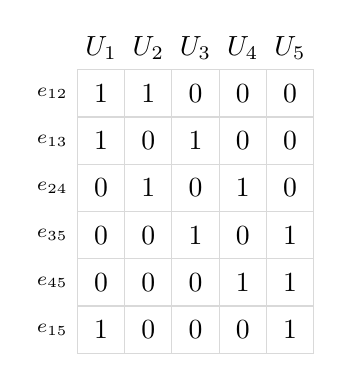
\begin{tikzpicture}[scale=0.6]
  \draw[step=1, gray!30, thin] (0,0) grid (5,6);
  \node at (0.5,5.5) {1}; \node at (1.5,5.5) {1}; \node at (2.5,5.5) {0}; \node at (3.5,5.5) {0}; \node at (4.5,5.5) {0};
  \node at (0.5,4.5) {1}; \node at (1.5,4.5) {0}; \node at (2.5,4.5) {1}; \node at (3.5,4.5) {0}; \node at (4.5,4.5) {0};
  \node at (0.5,3.5) {0}; \node at (1.5,3.5) {1}; \node at (2.5,3.5) {0}; \node at (3.5,3.5) {1}; \node at (4.5,3.5) {0};
  \node at (0.5,2.5) {0}; \node at (1.5,2.5) {0}; \node at (2.5,2.5) {1}; \node at (3.5,2.5) {0}; \node at (4.5,2.5) {1};
  \node at (0.5,1.5) {0}; \node at (1.5,1.5) {0}; \node at (2.5,1.5) {0}; \node at (3.5,1.5) {1}; \node at (4.5,1.5) {1};
  \node at (0.5,0.5) {1}; \node at (1.5,0.5) {0}; \node at (2.5,0.5) {0}; \node at (3.5,0.5) {0}; \node at (4.5,0.5) {1};
  \node[above] at (0.5,6) {$U_1$}; \node[above] at (1.5,6) {$U_2$}; \node[above] at (2.5,6) {$U_3$}; \node[above] at (3.5,6) {$U_4$}; \node[above] at (4.5,6) {$U_5$};
  \node[left, font=\scriptsize] at (0,5.5) {$e_{12}$}; \node[left, font=\scriptsize] at (0,4.5) {$e_{13}$}; \node[left, font=\scriptsize] at (0,3.5) {$e_{24}$};
  \node[left, font=\scriptsize] at (0,2.5) {$e_{35}$}; \node[left, font=\scriptsize] at (0,1.5) {$e_{45}$}; \node[left, font=\scriptsize] at (0,0.5) {$e_{15}$};
\end{tikzpicture}
\end{center}
\vspace{0.2em}
5 sites, 6 overlaps. Rank via Gaussian elimination over $\mathbb{F}_2$: $\rk(\partial_0) = 4$.\\$\rk H^1 = 6 - 4 = 2$ (if no triple overlaps contribute). Two independent obstructions.
\end{frame}

\begin{frame}{The Cover Builder in Detail}
\textbf{\texttt{cover\_builder.py}} constructs the Grothendieck cover from the CFG:

\begin{enumerate}\small
  \item \textbf{Node traversal}: Each CFG node $\to$ candidate site
  \item \textbf{Site classification}: Classify into 14 families by AST type
  \item \textbf{Overlap detection}: Two sites overlap if they share variables (value lineage) or control flow (dominator tree)
  \item \textbf{Boundary identification}: Input/output sites $\to$ boundary sections
  \item \textbf{Error site marking}: Division, index, attribute access $\to$ error sites
  \item \textbf{Morphism construction}: For each overlap, build a \texttt{ConcreteMorphism} with projection map
\end{enumerate}

\textbf{Result}: A \texttt{Cover} object ready for presheaf evaluation.
\end{frame}

\begin{frame}{SARIF Export: Integration with IDEs}
\textbf{SARIF} (Static Analysis Results Interchange Format): Standard for reporting static analysis results.

\vspace{0.3em}
Deppy's \texttt{sarif\_exporter.py} exports:
\begin{itemize}
  \item Each obstruction as a SARIF \texttt{result}
  \item Gap predicate in the \texttt{message}
  \item Repair guard in the \texttt{fix} suggestion
  \item Source location from \texttt{SiteId.source\_location}
  \item Severity from obstruction ranking
  \item $\rk H^1$ in the run-level \texttt{properties}
\end{itemize}

\vspace{0.2em}
This integrates with VS Code, GitHub Code Scanning, and any SARIF-compatible tool.
\end{frame}

\begin{frame}{Deppy's Contract Decorators}
\textbf{User-facing surface syntax} for specs:

\vspace{0.3em}
\begin{itemize}
  \item \texttt{@deppy.requires(lambda x: x > 0)} --- precondition
  \item \texttt{@deppy.ensures(lambda result: result >= 0)} --- postcondition
  \item \texttt{@deppy.invariant(lambda self: self.count >= 0)} --- class invariant
  \item \texttt{@deppy.decreases(lambda n: n)} --- termination measure
  \item \texttt{@deppy.theorem} --- user-supplied proof
  \item \texttt{@deppy.witness} --- constructive proof term
\end{itemize}

\vspace{0.2em}
Each decorator is lowered to a \texttt{BoundarySection} by the contract lowering pipeline. The sheaf machinery then checks if the function body satisfies the boundary constraints.
\end{frame}

\begin{frame}{The Bigger Picture: Programs as Spaces}
\textbf{The deep analogy:}

\vspace{0.3em}
\begin{center}
\renewcommand{\arraystretch}{1.4}
\begin{tabular}{@{}ll@{}}
\toprule
\textbf{Geometry} \& \textbf{Programming} \\
\midrule
Manifold \& Program \\
Open cover \& Code regions (sites) \\
Structure sheaf \& Type presheaf \\
Global section \& Consistent global typing \\
Tangent bundle \& Variable dependencies \\
Cohomology class \& Bug / obstruction \\
Euler characteristic \& Program health metric \\
Mayer-Vietoris \& Compositional analysis \\
Vector bundle \& Equivalence class \\
Descent \& Modular verification \\
\bottomrule
\end{tabular}
\end{center}

Programs \emph{are} spaces. Sheaf theory is the natural language for local-to-global reasoning about them.
\end{frame}

\begin{frame}{Final Thought}
\begin{center}
\vspace{1.5cm}
{\Large\textbf{``The sheaf condition is not a metaphor.\\It is the algorithm.''}}

\vspace{1.5cm}
{\normalsize Check gluing. Compute $H^1$. Count obstructions.\\Fix the minimum. Verify compositionality.\\That's it. That's the whole thing.}
\end{center}
\end{frame}
\end{document}
